% 2020 May 18 - THE MARTIAN ATMOSPHERIC BOUNDARY LAYER - https://agupubs.onlinelibrary.wiley.com/doi/10.1029/2010RG000351


%% Beginning of file 'sample63.tex'
%%
%% Modified 2019 June
%%
%% This is a sample manuscript marked up using the
%% AASTeX v6.3 LaTeX 2e macros.
%%
%% AASTeX is now based on Alexey Vikhlinin's emulateapj.cls 
%% (Copyright 2000-2015).  See the classfile for details.

%% AASTeX requires revtex4-1.cls (http://publish.aps.org/revtex4/) and
%% other external packages (latexsym, graphicx, amssymb, longtable, and epsf).
%% All of these external packages should already be present in the modern TeX 
%% distributions.  If not they can also be obtained at www.ctan.org.

%% The first piece of markup in an AASTeX v6.x document is the \documentclass
%% command. LaTeX will ignore any data that comes before this command. The 
%% documentclass can take an optional argument to modify the output style.
%% The command below calls the preprint style which will produce a tightly 
%% typeset, one-column, single-spaced document.  It is the default and thus
%% does not need to be explicitly stated.
%%
%%
%% using aastex version 6.3
\usepackage{amsmath}
\documentclass{aastex63}

%% The default is a single spaced, 10 point font, single spaced article.
%% There are 5 other style options available via an optional argument. They
%% can be invoked like this:
%%
%% \documentclass[arguments]{aastex63}
%% 
%% where the layout options are:
%%
%%  twocolumn   : two text columns, 10 point font, single spaced article.
%%                This is the most compact and represent the final published
%%                derived PDF copy of the accepted manuscript from the publisher
%%  manuscript  : one text column, 12 point font, double spaced article.
%%  preprint    : one text column, 12 point font, single spaced article.  
%%  preprint2   : two text columns, 12 point font, single spaced article.
%%  modern      : a stylish, single text column, 12 point font, article with
%% 		  wider left and right margins. This uses the Daniel
%% 		  Foreman-Mackey and David Hogg design.
%%  RNAAS       : Preferred style for Research Notes which are by design 
%%                lacking an abstract and brief. DO NOT use \begin{abstract}
%%                and \end{abstract} with this style.
%%
%% Note that you can submit to the AAS Journals in any of these 6 styles.
%%
%% There are other optional arguments one can invoke to allow other stylistic
%% actions. The available options are:
%%
%%   astrosymb    : Loads Astrosymb font and define \astrocommands. 
%%   tighten      : Makes baselineskip slightly smaller, only works with 
%%                  the twocolumn substyle.
%%   times        : uses times font instead of the default
%%   linenumbers  : turn on lineno package.
%%   trackchanges : required to see the revision mark up and print its output
%%   longauthor   : Do not use the more compressed footnote style (default) for 
%%                  the author/collaboration/affiliations. Instead print all
%%                  affiliation information after each name. Creates a much 
%%                  longer author list but may be desirable for short 
%%                  author papers.
%% twocolappendix : make 2 column appendix.
%%   anonymous    : Do not show the authors, affiliations and acknowledgments 
%%                  for dual anonymous review.
%%
%% these can be used in any combination, e.g.
%%
%% \documentclass[twocolumn,linenumbers,trackchanges]{aastex63}
%%
%% AASTeX v6.* now includes \hyperref support. While we have built in specific
%% defaults into the classfile you can manually override them with the
%% \hypersetup command. For example,
%%
%% \hypersetup{linkcolor=red,citecolor=green,filecolor=cyan,urlcolor=magenta}
%%
%% will change the color of the internal links to red, the links to the
%% bibliography to green, the file links to cyan, and the external links to
%% magenta. Additional information on \hyperref options can be found here:
%% https://www.tug.org/applications/hyperref/manual.html#x1-40003
%%
%% Note that in v6.3 "bookmarks" has been changed to "true" in hyperref
%% to improve the accessibility of the compiled pdf file.
%%
%% If you want to create your own macros, you can do so
%% using \newcommand. Your macros should appear before
%% the \begin{document} command.
%%
\newcommand{\vdag}{(v)^\dagger}
\newcommand\aastex{AAS\TeX}
\newcommand\latex{La\TeX}

%% Reintroduced the \received and \accepted commands from AASTeX v5.2
\received{June 1, 2019}
\revised{January 10, 2019}
\accepted{\today}
%% Command to document which AAS Journal the manuscript was submitted to.
%% Adds "Submitted to " the argument.
\submitjournal{PSJ}

%% For manuscript that include authors in collaborations, AASTeX v6.3
%% builds on the \collaboration command to allow greater freedom to 
%% keep the traditional author+affiliation information but only show
%% subsets. The \collaboration command now must appear AFTER the group
%% of authors in the collaboration and it takes TWO arguments. The last
%% is still the collaboration identifier. The text given in this
%% argument is what will be shown in the manuscript. The first argument
%% is the number of author above the \collaboration command to show with
%% the collaboration text. If there are authors that are not part of any
%% collaboration the \nocollaboration command is used. This command takes
%% one argument which is also the number of authors above to show. A
%% dashed line is shown to indicate no collaboration. This example manuscript
%% shows how these commands work to display specific set of authors 
%% on the front page.
%%
%% For manuscript without any need to use \collaboration the 
%% \AuthorCollaborationLimit command from v6.2 can still be used to 
%% show a subset of authors.
%
%\AuthorCollaborationLimit=2
%
%% will only show Schwarz & Muench on the front page of the manuscript
%% (assuming the \collaboration and \nocollaboration commands are
%% commented out).
%%
%% Note that all of the author will be shown in the published article.
%% This feature is meant to be used prior to acceptance to make the
%% front end of a long author article more manageable. Please do not use
%% this functionality for manuscripts with less than 20 authors. Conversely,
%% please do use this when the number of authors exceeds 40.
%%
%% Use \allauthors at the manuscript end to show the full author list.
%% This command should only be used with \AuthorCollaborationLimit is used.

%% The following command can be used to set the latex table counters.  It
%% is needed in this document because it uses a mix of latex tabular and
%% AASTeX deluxetables.  In general it should not be needed.
%\setcounter{table}{1}

%%%%%%%%%%%%%%%%%%%%%%%%%%%%%%%%%%%%%%%%%%%%%%%%%%%%%%%%%%%%%%%%%%%%%%%%%%%%%%%%
%%
%% The following section outlines numerous optional output that
%% can be displayed in the front matter or as running meta-data.
%%
%% If you wish, you may supply running head information, although
%% this information may be modified by the editorial offices.
\shorttitle{Vortices and Meteorology from Insight}
\shortauthors{Jackson}
%%
%% You can add a light gray and diagonal water-mark to the first page 
%% with this command:
%% \watermark{text}
%% where "text", e.g. DRAFT, is the text to appear.  If the text is 
%% long you can control the water-mark size with:
%% \setwatermarkfontsize{dimension}
%% where dimension is any recognized LaTeX dimension, e.g. pt, in, etc.
%%
%%%%%%%%%%%%%%%%%%%%%%%%%%%%%%%%%%%%%%%%%%%%%%%%%%%%%%%%%%%%%%%%%%%%%%%%%%%%%%%%
\graphicspath{{./}{figures/}}
%% This is the end of the preamble.  Indicate the beginning of the
%% manuscript itself with \begin{document}.

\begin{document}

\title{Inferring Vortex and Meteorological Statistics from Insight}

%% LaTeX will automatically break titles if they run longer than
%% one line. However, you may use \\ to force a line break if
%% you desire. In v6.3 you can include a footnote in the title.

%% A significant change from earlier AASTEX versions is in the structure for 
%% calling author and affiliations. The change was necessary to implement 
%% auto-indexing of affiliations which prior was a manual process that could 
%% easily be tedious in large author manuscripts.
%%
%% The \author command is the same as before except it now takes an optional
%% argument which is the 16 digit ORCID. The syntax is:
%% \author[xxxx-xxxx-xxxx-xxxx]{Author Name}
%%
%% This will hyperlink the author name to the author's ORCID page. Note that
%% during compilation, LaTeX will do some limited checking of the format of
%% the ID to make sure it is valid. If the "orcid-ID.png" image file is 
%% present or in the LaTeX pathway, the OrcID icon will appear next to
%% the authors name.
%%
%% Use \affiliation for affiliation information. The old \affil is now aliased
%% to \affiliation. AASTeX v6.3 will automatically index these in the header.
%% When a duplicate is found its index will be the same as its previous entry.
%%
%% Note that \altaffilmark and \altaffiltext have been removed and thus 
%% can not be used to document secondary affiliations. If they are used latex
%% will issue a specific error message and quit. Please use multiple 
%% \affiliation calls for to document more than one affiliation.
%%
%% The new \altaffiliation can be used to indicate some secondary information
%% such as fellowships. This command produces a non-numeric footnote that is
%% set away from the numeric \affiliation footnotes.  NOTE that if an
%% \altaffiliation command is used it must come BEFORE the \affiliation call,
%% right after the \author command, in order to place the footnotes in
%% the proper location.
%%
%% Use \email to set provide email addresses. Each \email will appear on its
%% own line so you can put multiple email address in one \email call. A new
%% \correspondingauthor command is available in V6.3 to identify the
%% corresponding author of the manuscript. It is the author's responsibility
%% to make sure this name is also in the author list.
%%
%% While authors can be grouped inside the same \author and \affiliation
%% commands it is better to have a single author for each. This allows for
%% one to exploit all the new benefits and should make book-keeping easier.
%%
%% If done correctly the peer review system will be able to
%% automatically put the author and affiliation information from the manuscript
%% and save the corresponding author the trouble of entering it by hand.

\correspondingauthor{Brian Jackson}
\email{bjackson@boisestate.edu}

\author[0000-0002-9495-9700]{Brian Jackson}
\author{Justin Crevier}
\author{Michelle Szurgot}
\author{Ryan Battin}
\affiliation{Department of Physics\\ 
Boise State University\\ 
1910 University Drive, Boise ID 83725-1570 USA}

%% Note that the \and command from previous versions of AASTeX is now
%% depreciated in this version as it is no longer necessary. AASTeX 
%% automatically takes care of all commas and "and"s between authors names.

%% AASTeX 6.3 has the new \collaboration and \nocollaboration commands to
%% provide the collaboration status of a group of authors. These commands 
%% can be used either before or after the list of corresponding authors. The
%% argument for \collaboration is the collaboration identifier. Authors are
%% encouraged to surround collaboration identifiers with ()s. The 
%% \nocollaboration command takes no argument and exists to indicate that
%% the nearby authors are not part of surrounding collaborations.

%% Mark off the abstract in the ``abstract'' environment. 
\begin{abstract}
The Insight Mission has operated on the surface of Mars for nearly two Earth years, returning hundreds of sols worth of data, including detections of the first Marsquakes. The lander also deployed an exquisitely sensitive meteorological instrument package to assess the influence of the atmosphere on the geophysical measurements, as well as imaging cameras to monitor both instrument deployment and local surface activity. In addition to their relevance to Insight geoscience, these latter instruments have detected a variety of boundary layer phenomena, including an unprecedented number of encounters with small-scale vortices. These vortices register as short-lived ($<$ tens of seconds), negative ($<$ a few \% ambient) pressure excursions in the barometric time-series collected by Insight. These vortices closely resemble dust devils, which largely shape climate and air quality on Mars where they are widespread. Puzzlingly, although Insight detected more than 9,000 such vortices and collected hundreds of mid-day images (as reported in \citealp{2020arXiv200501134S}), no active dust devils were imaged -- apparently, all the vortices were dustless. In spite of the lack of dust devil detections, we can leverage the vortex detections and Insight’s daily wind speed measurements to learn about the boundary layer processes that create dust devils. Such an analysis could even help us optimize our vortex detection strategies. In this study, we will discuss our own analysis of Insight’s meteorological data to assess the statistics of vortex and dust devil activity. Comparing these results to Insight’s imagery and space-based observations of the Insight landing site, we can also statistically infer the maximum dust-loading allowed for nearby dust devils. 
\end{abstract}

%% Keywords should appear after the \end{abstract} command. 
%% See the online documentation for the full list of available subject
%% keywords and the rules for their use.
\keywords{editorials, notices --- 
miscellaneous --- catalogs --- surveys}

%% From the front matter, we move on to the body of the paper.
%% Sections are demarcated by \section and \subsection, respectively.
%% Observe the use of the LaTeX \label
%% command after the \subsection to give a symbolic KEY to the
%% subsection for cross-referencing in a \ref command.
%% You can use LaTeX's \ref and \label commands to keep track of
%% cross-references to sections, equations, tables, and figures.
%% That way, if you change the order of any elements, LaTeX will
%% automatically renumber them.
%%
%% We recommend that authors also use the natbib \citep
%% and \citet commands to identify citations.  The citations are
%% tied to the reference list via symbolic KEYs. The KEY corresponds
%% to the KEY in the \bibitem in the reference list below. 

\section{Introduction} \label{sec:Introduction}

% 2020 May 16 - Discuss how Greeley et al. (2006) spotted and analyzed dust devils.

% \citet{2010Icar..206..306N} report a dust flux $Q$ that depends on the pressure deficit at the center of a vortex $\Delta P$ as
% \begin{equation}
%     Q = \left(5.79\times10^{-8} {\rm kg\ m^{-2}\ s^{-1}} \right) \left( \Delta P/{\rm Pa}\right)^{3.40}.
%     \label{eqn:Neakrase_dust_flux}
% \end{equation}
% \begin{figure}
%     \centering
%     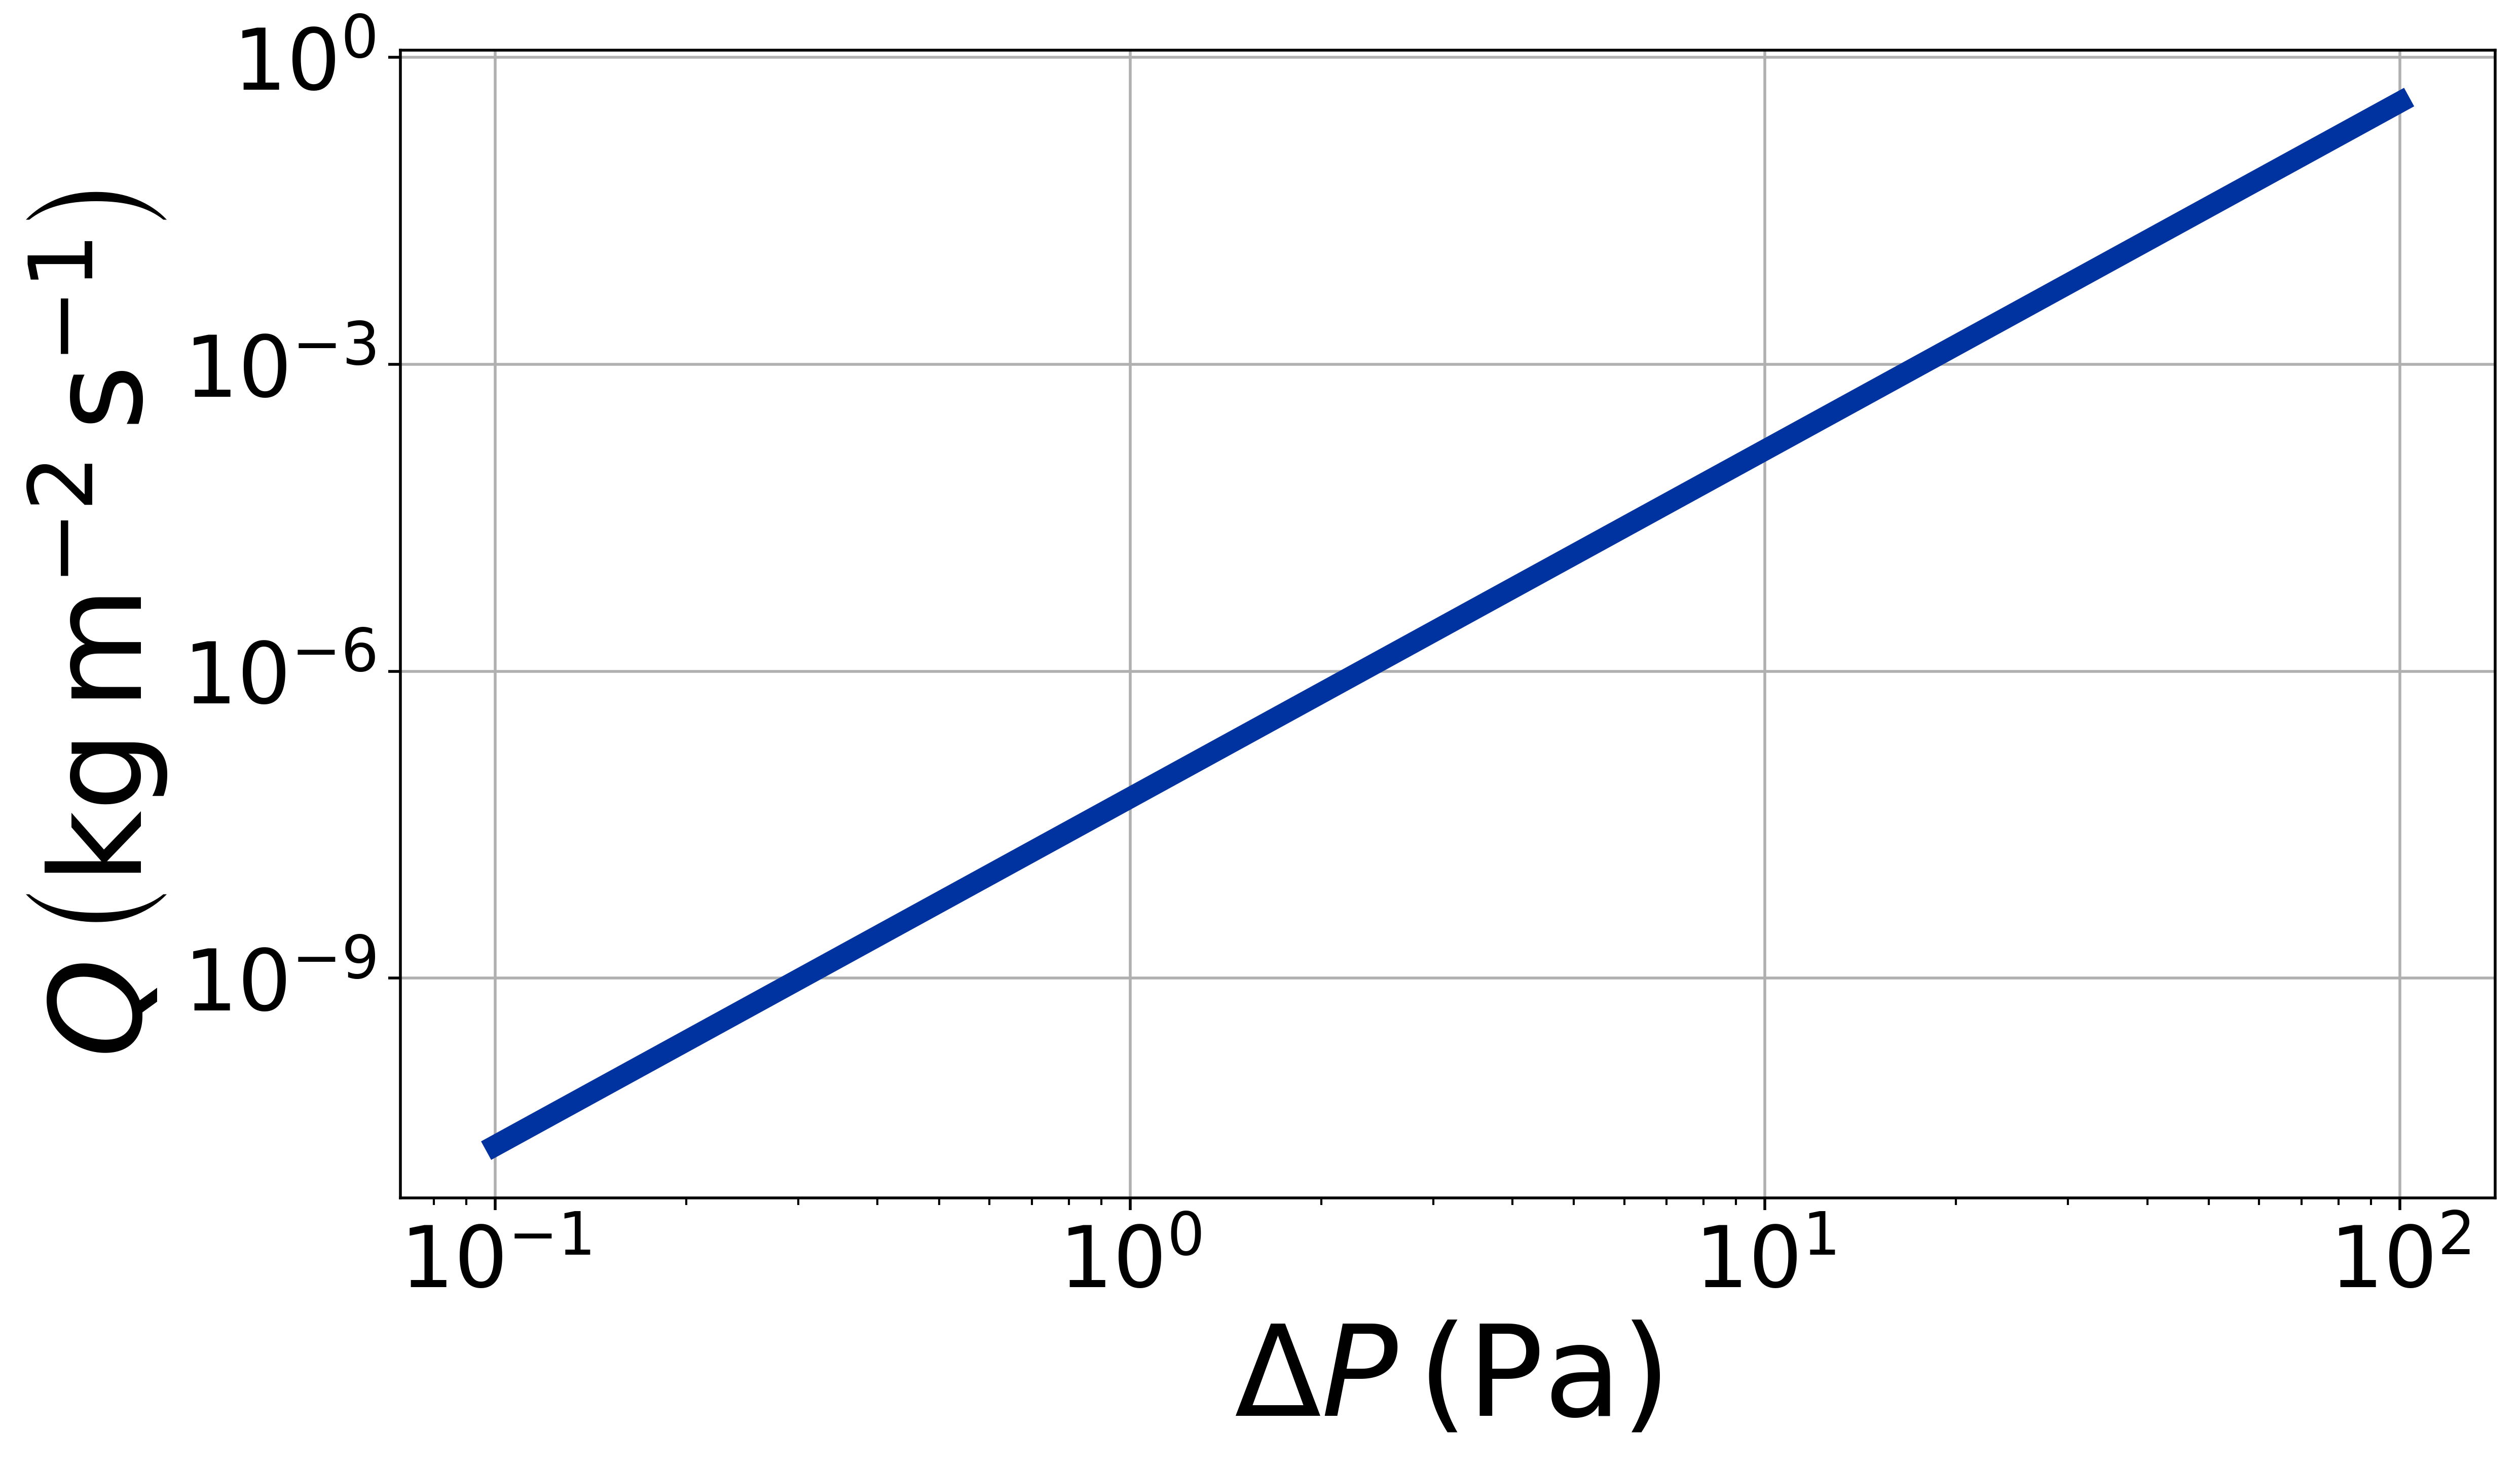
\includegraphics[width=\textwidth]{figures/Q_vs_Delta-P.png}
%     \caption{Dust flux $Q$ as a function of the pressure dip at the center of a lab-generated vortex $\Delta P$, as reported in \citet{2010Icar..206..306N}.}
%     \label{fig:Neakrase_dust_flux}
% \end{figure}

An in-situ survey could be tailored to test ideas about dust devils. 

\citet{1998JAtS...55.3244R} proposed the ``dust devil activity'' (DDA) parameter, the product of the surface sensible heat flux and a thermodynamic efficiency related to the depth of the planetary boundary layer. During the martian day, the heat flux and boundary layer depth increase as insolation heats the surface. \citet{2019JGRE..124.3442N} conducted large eddy simulations of the environment in and around Gale Crater to assess the DDA, along with other micrometeorological parameters as a function of position and time-of-day. The study then compared those model predictions to the rate at which short-lived dips appeared in the barometric time-series, likely indicative of vortex encounters. The study found that the frequency of vortex encounters scaled with DDA.

However, in \citet{1998JAtS...55.3244R}, the actual relationship between DDA and dust devil properties remains unclear: whether a larger DDA translates into a higher frequency of dust devils, more large dust devils, more vigorous dust devils. The results in \citet{2019JGRE..124.3442N} suggest the frequency at least increases with DDA, but it is not clear whether the increased frequency arose from higher surface winds (which would more quickly advect vortices past the sensor). Also unknown was whether the detected vortices exhibited deeper pressure excursions or more vigorous winds. A tailored imaging survey for dust devils, especially combined with a meteorological dataset, could disentangle the influence of DDA on dust devil properties. 

The detailed influence of dust devils on Mars' atmosphere likewise remain obscure. 

For this study, we will consider two types of dust devil detections and analyses: the first involves dust devils far enough from the instrument suite that they are analyzed using only imagery; the second involves dust devils that pass over the instruments. The latter detection has the potential to more directly elucidate the pressure, temperature, and wind structures within a dust devil, as well as the dust abundance but requires a rare encounter at a distance from a devil's center not much more than the eyewall diameter. The former detection may also reveal the dust content but indirectly, via a analysis of the image contrast; however such detections are much more common since they can be made out to the resolution of the imaging system and may therefore provide a more robust assessment of dust devil statistics. 

% Define areal density N

The atmospheric influence of a dust devil population depends on the areal density of dust devil occurrence and the dust flux for each. Thus, accurately assessing that influence requires accurate estimates of the both.

\section{Pressure Time-Series Data and Analysis}
We analyze the pressure time-series collected by Insight's Auxiliary Payload Sensor Subsystem or APSS, which measures the local magnetic field, wind, and atmospheric temperature, in addition to ambient pressure. 

As in previous work \citep[e.g.][]{2016JGRE..121.1514K}, we model the vortex signals using a steady-state modified Lorentzian profile $L(t)$:
\begin{equation}
    L(t) = \frac{-\Delta P_{\rm obs}}{1 + \left( \frac{ t - t_0 }{\Gamma_{\rm obs}/2} \right)^2},\label{eqn:Lorentzian_profile}
\end{equation}
where $t$ is the time of each datum, $\Delta P_{\rm obs}$ is the maximum pressure excursion observed (a positive number) at the center of vortex signal, $t_0$ the central time, and $\Gamma_{\rm obs}$ the observed profile full-width/half-max (FWHM). This profile assumes the vortex travels past the sensor on a simple linear trajectory with a unidirectional and constant velocity $U$. 

In addition to vortex signals and Gaussian (white) noise, the data also exhibit long-term variations of timescales typically much longer (minutes to hours) than the vortex signals. To suppress these longer-term signals and facilitate detection of the vortices, we apply a mean boxcar filter with a window size $W$ before sifting the data for vortices. Next, to recover the pressure signatures of vortices, we employ a matched filter approach \citep[][ch.~13]{Press2007}; that is, we march a Lorentzian profile, point-by-point, across the time series, convolving it with the time-series. This process produces the equivalent of a spectrum, with large positive spikes when the filter encounters other Lorentzian-like shapes. Any time-series analysis scheme will unavoidably involve selection effects that can skew the recovered population of signals \citep{2018Icar..299..166J}, so, in addition to outlining our approach here, we explore its biases and how those influence the final recovered population of vortices below.




Most observed vortices pass near but directly over the sensor, i.e., they have a non-zero miss distance $b$. If, instead, the center of a vortex passed directly over the sensor, it would register central pressure excursion (the ``actual'' value $P_{\rm act}$), and the profile FWHM would relate directly to the vortex diameter $D_{\rm act}$ and speed (i.e., $\Gamma_{\rm act} = U D_{\rm act}$). If the wind profile is measured simultaneously with the pressure profile, then $b$ may be estimated, as well as $P_{\rm act}$ and $D_{\rm act}$ \citep{2016Icar..271..326L, 2020AeoRe..4400594F}. Otherwise, the observed profile depth and width ($P_{\rm obs}$ and $\Gamma_{\rm obs}$) are smaller and larger, respectively, than their actual values with consequences to estimates for meteorological impacts of vortices and dust devils \citep{2018Icar..299..166J, 2019Icar..317..209K}.

Usually, the pressure time-series is conditioned so it consists primarily of vortex passages and roughly white noise (with a variance $\sigma_{\rm P}^2$). Detection schemes can then sift the pressure time-series for individual outlier points with minimum threshold pressure excursions $\Delta P_{\rm obs} \geq \Delta P_{\rm min}$ some multiple of $\sigma_{\rm P}$ \citep{2010JGRE..115.0E16E, 2020arXiv200501134S}. 

these distortion effects influence the recovery of an underlying vortex population? As an example, assume all vortices have the same $\Delta P_{\rm act}$- and $D_{\rm act}$-values -- typical values for Mars are $\Delta P_{\rm act} = 0.5\,{\rm Pa}$ and $D_{\rm act} = 50\,{\rm m}$. With $U = 5\,{\rm m\ s^{-1}}$, $\Gamma_{\rm act} = 10\, {\rm s}$. (In reality, these parameters exhibit a wide but highly skewed distribution, rendering ``typical'' values of dubious merit -- \citealp{2016SSRv..203..277L}.) Usually, the pressure time-series is conditioned so it consists primarily of vortex passages and roughly white noise (with a variance $\sigma_{\rm P}^2$). Detection schemes can then sift the pressure time-series for individual outlier points with minimum threshold pressure excursions $\Delta P_{\rm obs} \geq \Delta P_{\rm min}$ some multiple of $\sigma_{\rm P}$ \citep{2010JGRE..115.0E16E, 2020arXiv200501134S}. Assume, therefore, that all vortices that pass within a certain maximum distance $b_{\rm max}$ are detected, with
\begin{equation}
    b_{\rm max} = \left( \frac{D_{\rm act}}{2} \right) \sqrt{ \frac{\Delta P_{\rm act}}{\Delta P_{\rm min}} - 1 } \label{eqn:bmax},
\end{equation} 
where we take $P_{\rm act} \gg P_{\rm min}$ for simplicity.

With an areal density $N$ measured in per unit area, the total number of vortices probed $k$ is given by 
\begin{equation}
    k = 2 N U T b_{\rm max} = N U T D_{\rm act} \sqrt{ \frac{\Delta P_{\rm act}}{\Delta P_{\rm min}} - 1 }, \label{eqn:number_of_encounters}
\end{equation}
where $T$ is the total duration of the survey (which may consist of multiple observational sequences spread over many sols). If $N$ and $U$ evolve with time (as they usually do), this estimate can be converted into an integral over time. As an example, \citet{2020arXiv200501134S} take $\Delta P_{\rm min} = 0.3\,{\rm Pa}$ and report vortex activity spanning about 12 hours ($ = T$) each sol. Taking $N \approx 1\,{\rm km^{-2}}$ \citep{2016SSRv..203..277L}, Equation \ref{eqn:number_of_encounters} suggests a daily encounter rate of about 16 vortices, which compares favorably to the daily rates reported in \citet{2020arXiv200501134S}. Equation \ref{eqn:bmax} suggests these detections originate from vortices that pass within $b_{\rm max} = 20\,{\rm m}$ of the Insight lander.

\citet{2018SSRv..214..109S} and \citet{2020NatGe..13..190B} provide details of the instrument calibration and operation. 

Of course, any time-series analysis will unavoidably involve selection effects that can skew the recovered population of signals \citep{2018Icar..299..166J}, so, in addition to outlining our approach here, we explore its biases and how those influence the final recover population of vortices in Section XXX.

% Show how mean boxcar with a given window size distorts Lorentzian

% Discuss how the matched filter works

\section{Results and Discussion}

If $b = 0$, then the center of the given vortex passes directly over the barometer and the observed profile will exactly match the actual profile. However, such a central encounter has vanishing probability \citep{2018Icar..299..166J, 2019Icar..317..209K}. Consequently, the observed profile parameters are given by
\begin{equation}
    \Delta P_{\rm obs} &=& \frac{\Delta P_{\rm act}}{1 + \left( 2b/D_{\rm act} \right)^2 }\label{eqn:Pobs}
\end{equation}
and
\begin{equation}
    \Gamma_{\rm obs} &=& \sqrt{\Gamma_{\rm act}^2  + \left(2 b \right)^2}.\label{eqn:Gammaobs}
\end{equation}
Another useful relationship is given by 
\begin{equation}
    \Delta P_{\rm obs} \Gamma_{\rm obs}^2 = \Delta P_{\rm act} \Gamma_{\rm act}^2.\label{eqn:conservation_eqn}
\end{equation}
Taken together, these equations mean that the observed profile in the barometric time-series will usually be skewed shallower ($\Delta P_{\rm obs} < \Delta P_{\rm act}$) and broader ($\Gamma_{\rm obs} > \Gamma_{\rm act}$) than the actual profile. Since $b$ is usually unknown, it is not usually possible to determine how much shallower and broader, though \citep{2018Icar..299..166J, 2019Icar..317..209K}. (If the wind profile is measured simultaneously, though, $b$ may be estimated -- \citealp{2016Icar..271..326L, 2020AeoRe..4400594F}.)

How do these distortion effects influence the recovery of an underlying vortex population? As an example, assume all vortices have the same $\Delta P_{\rm act}$- and $D_{\rm act}$-values -- typical values for Mars are $\Delta P_{\rm act} = 0.5\,{\rm Pa}$ and $D_{\rm act} = 50\,{\rm m}$. With $U = 5\,{\rm m\ s^{-1}}$, $\Gamma_{\rm act} = 10\, {\rm s}$. (In reality, these parameters exhibit a wide but highly skewed distribution, rendering ``typical'' values of dubious merit -- \citealp{2016SSRv..203..277L}.) Usually, the pressure time-series is conditioned so it consists primarily of vortex passages and roughly white noise (with a variance $\sigma_{\rm P}^2$). Detection schemes can then sift the pressure time-series for individual outlier points with minimum threshold pressure excursions $\Delta P_{\rm obs} \geq \Delta P_{\rm min}$ some multiple of $\sigma_{\rm P}$ \citep{2010JGRE..115.0E16E, 2020arXiv200501134S}. Assume, therefore, that all vortices that pass within a certain maximum distance $b_{\rm max}$ are detected, with
\begin{equation}
    b_{\rm max} = \left( \frac{D_{\rm act}}{2} \right) \sqrt{ \frac{\Delta P_{\rm act}}{\Delta P_{\rm min}} - 1 } \label{eqn:bmax},
\end{equation} 
where we take $P_{\rm act} \gg P_{\rm min}$ for simplicity.

With an areal density $N$ measured in per unit area, the total number of vortices probed $k$ is given by 
\begin{equation}
    k = 2 N U T b_{\rm max} = N U T D_{\rm act} \sqrt{ \frac{\Delta P_{\rm act}}{\Delta P_{\rm min}} - 1 }, \label{eqn:number_of_encounters}
\end{equation}
where $T$ is the total duration of the survey (which may consist of multiple observational sequences spread over many sols). If $N$ and $U$ evolve with time (as they usually do), this estimate can be converted into an integral over time. As an example, \citet{2020arXiv200501134S} take $\Delta P_{\rm min} = 0.3\,{\rm Pa}$ and report vortex activity spanning about 12 hours ($ = T$) each sol. Taking $N \approx 1\,{\rm km^{-2}}$ \citep{2016SSRv..203..277L}, Equation \ref{eqn:number_of_encounters} suggests a daily encounter rate of about 16 vortices, which compares favorably to the daily rates reported in \citet{2020arXiv200501134S}. Equation \ref{eqn:bmax} suggests these detections originate from vortices that pass within $b_{\rm max} = 20\,{\rm m}$ of the Insight lander.

Another typical feature of detection schemes: $\Gamma_{\rm obs} < \Gamma_{\rm max}$, with $\Gamma_{\rm max} \sim 1000\,{\rm s}$. 

We can estimate the reduction in the pressure excursion $\Delta P_{\rm obs}^\prime$ that results from applying a mean boxcar filter of width $W$ as 
\begin{equation}
    \Delta P_{\rm obs}^\prime = -\frac{1}{W} \int_{-1/2 W}^{1/2 W} \frac{\Delta P_{\rm obs}}{1 + \left( 2t/\Gamma_{\rm obs} \right)^2} dt = -\Delta P_{\rm obs} \left( \frac{\Gamma_{\rm obs}}{W} \right) \tan^{-1} \left( \frac{W}{\Gamma_{\rm obs}} \right).\label{eqn:Pobsprime}
\end{equation}

As discussed in Section \ref{sec:Introduction}, the quantity of meteorological interest is $N$, which can be estimated from this equation. In particular, we can test predictions for how $N$ should vary with ambient conditions (sensible heat flux, ambient wind speed and shear, boundary layer depth, etc. -- \citealp{2019JGRE..124.3442N}) but only to the extent that we can reliably distinguish different values for $N$. This requirement necessitates an estimate for the uncertainty associated with any estimate of $N$. A reasonable assumption is that vortex encounters represent a Poisson process \citep[cf.][]{Press2007}. We can estimate the uncertainty on $k$ as $\sigma_k = \sqrt{k}$ and therefrom the uncertainty $\sigma_N$ via
\begin{equation}
    \frac{\sigma_N}{N} = \frac{\sigma_k}{k} = k^{-1/2} = \left ( N U T D_{\rm act} \right)^{-1/2} \left( \frac{\Delta P_{\rm act}}{\Delta P_{\rm min}} - 1 \right)^{-1/4}.
    \label{eqn:sigma_N}
\end{equation}

\section{Camera Model}
To begin with, we outline the very basic characteristics of our model camera. By design, the considerations here are simplistic and general, rendering them applicable to a wide range of imaging systems. Consider a camera angled to have a clear view of the horizon and with a horizontal field-of-view $\Delta_{\rm FOV}$ centered on azimuth $\lambda$ and an angular resolution $\alpha$ measured in angle per pixel (Figure \ref{fig:Awedge}). Consider also a dust devil with a fixed diameter $D$, height $H$, and a sufficient contrast against the image background that it can be detected. Such a dust devil could be resolved at a distance from the camera $r_{\rm max} = D/\alpha$. For example, to resolve a dust devil with $D = 10\,{\rm m}$ with three pixels across, if $\alpha = 0.3\,{\rm mrad\ pix^{-1}} \times 3\,{\rm pix} \approx 1\,{\rm mrad}$ (similar to the Mars 2020 Mastcam-Z - \citealp{2017E&SS....4..396B}), $r_{\rm max} \approx 10\,{\rm km}$.

\begin{figure}
    \centering
    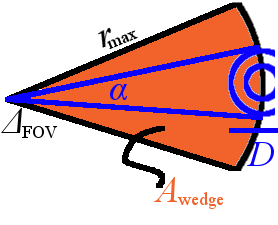
\includegraphics[width=0.5\textwidth]{figures/Awedge.jpg}
    \caption{Observational geometry. The camera has a field-of-view is $\Delta_{\rm FOV}$ and an angular resolution $\alpha$ which allows it to resolve dust devils of diameter $D$ out to a radial distance $r_{\rm max}$. The area surveyed is $A_{\rm wedge}$.}
    \label{fig:Awedge}
\end{figure}

In principle, the camera could detect this dust devil if it traversed the pie-wedge of terrain centered on $\lambda$ and having an area 
\begin{equation}
    A_{\rm wedge} = \frac{\Delta_{\rm FOV} r_{\rm max}^2}{2} = \frac{\Delta_{\rm FOV}D^2}{2 \alpha^2}.
    \label{eqn:A_wedge}
\end{equation}
Taking the same $D$ and $\alpha$-values as above, along with $\Delta_{\rm FOV} = \pi/2\,{\rm rad}$ gives $A_{\rm wedge} \sim 100\,{\rm km^2}$. If dust devils traveled very slowly (or not at all) from their origin point, then the survey would only include devils that appeared within this wedge. However, as pointed out in \citet{2014JAtS...71.4461L}, advection of dust devils through a survey site increases the effective area surveyed. 

Consider a fixed, unidirectional wind of speed $U$ crossing perpendicularly through the pie-wedge. If the dust devil under consideration has a lifetime $\tau$, then it will travel a distance $L = \tau U$ before dissipating. Thus, the wind field can advect dust devils into the camera's field-of-view acting as a conveyor belt with area
\begin{equation}
    A_{\rm adv} = r_{\rm max} L = \frac{D U \tau}{\alpha}.
    \label{eqn:A_adv}
\end{equation}
Again, typical values $D \sim 10\,{\rm m}$, $U \sim 10\,{\rm m\ s^{-1}}$, $\tau \sim 100\,{\rm s}$, and $\alpha \sim 1\,{\rm mrad}$ gives $A_{\rm adv} \sim 10\,{\rm km^2} \ll A_{\rm wedge}$. Although both areas contribute, we neglect $A_{\rm adv}$ compared to $A_{\rm wedge}$, and we use this estimate for the area surveyed $A_{\rm survey} \approx A_{\rm wedge}$ to determine how the inferred population of dust devils depends on the survey parameters.

\section{Imaging Surveys for Distant Dust Devils}
First, we consider the accuracy with which we could infer the occurrence rate of dust devils detected very distant from the instrument suite and that register only on the camera instrument. We can relate the areal density $N$ (dust devils per unit area) for a certain period of interest from the total number of dust devils observed in a single image $k$:
\begin{equation}
   N = \frac{k}{A_{\rm survey}} = \left( \frac{2 \alpha^2}{\Delta_{\rm FOV} D^2} \right)\ k.
    \label{eqn:areal_occurrence}
\end{equation}

If we assume that dust devil occurrence is a Poisson process, then we can estimate the standard deviation or uncertainty on $k$ as $\sigma_k = \sqrt{k}$ and the uncertainty $\sigma_N$ on our estimate of $N$ via
\begin{equation}
    \frac{\sigma_N}{N} = \frac{\sigma_k}{k} = k^{-1/2} = \sqrt{2} N^{-1/2} D^{-1}\ \Delta_{\rm FOV}^{-1/2} \alpha.
    \label{eqn:sigma_N}
\end{equation}

\begin{figure}
    \centering
    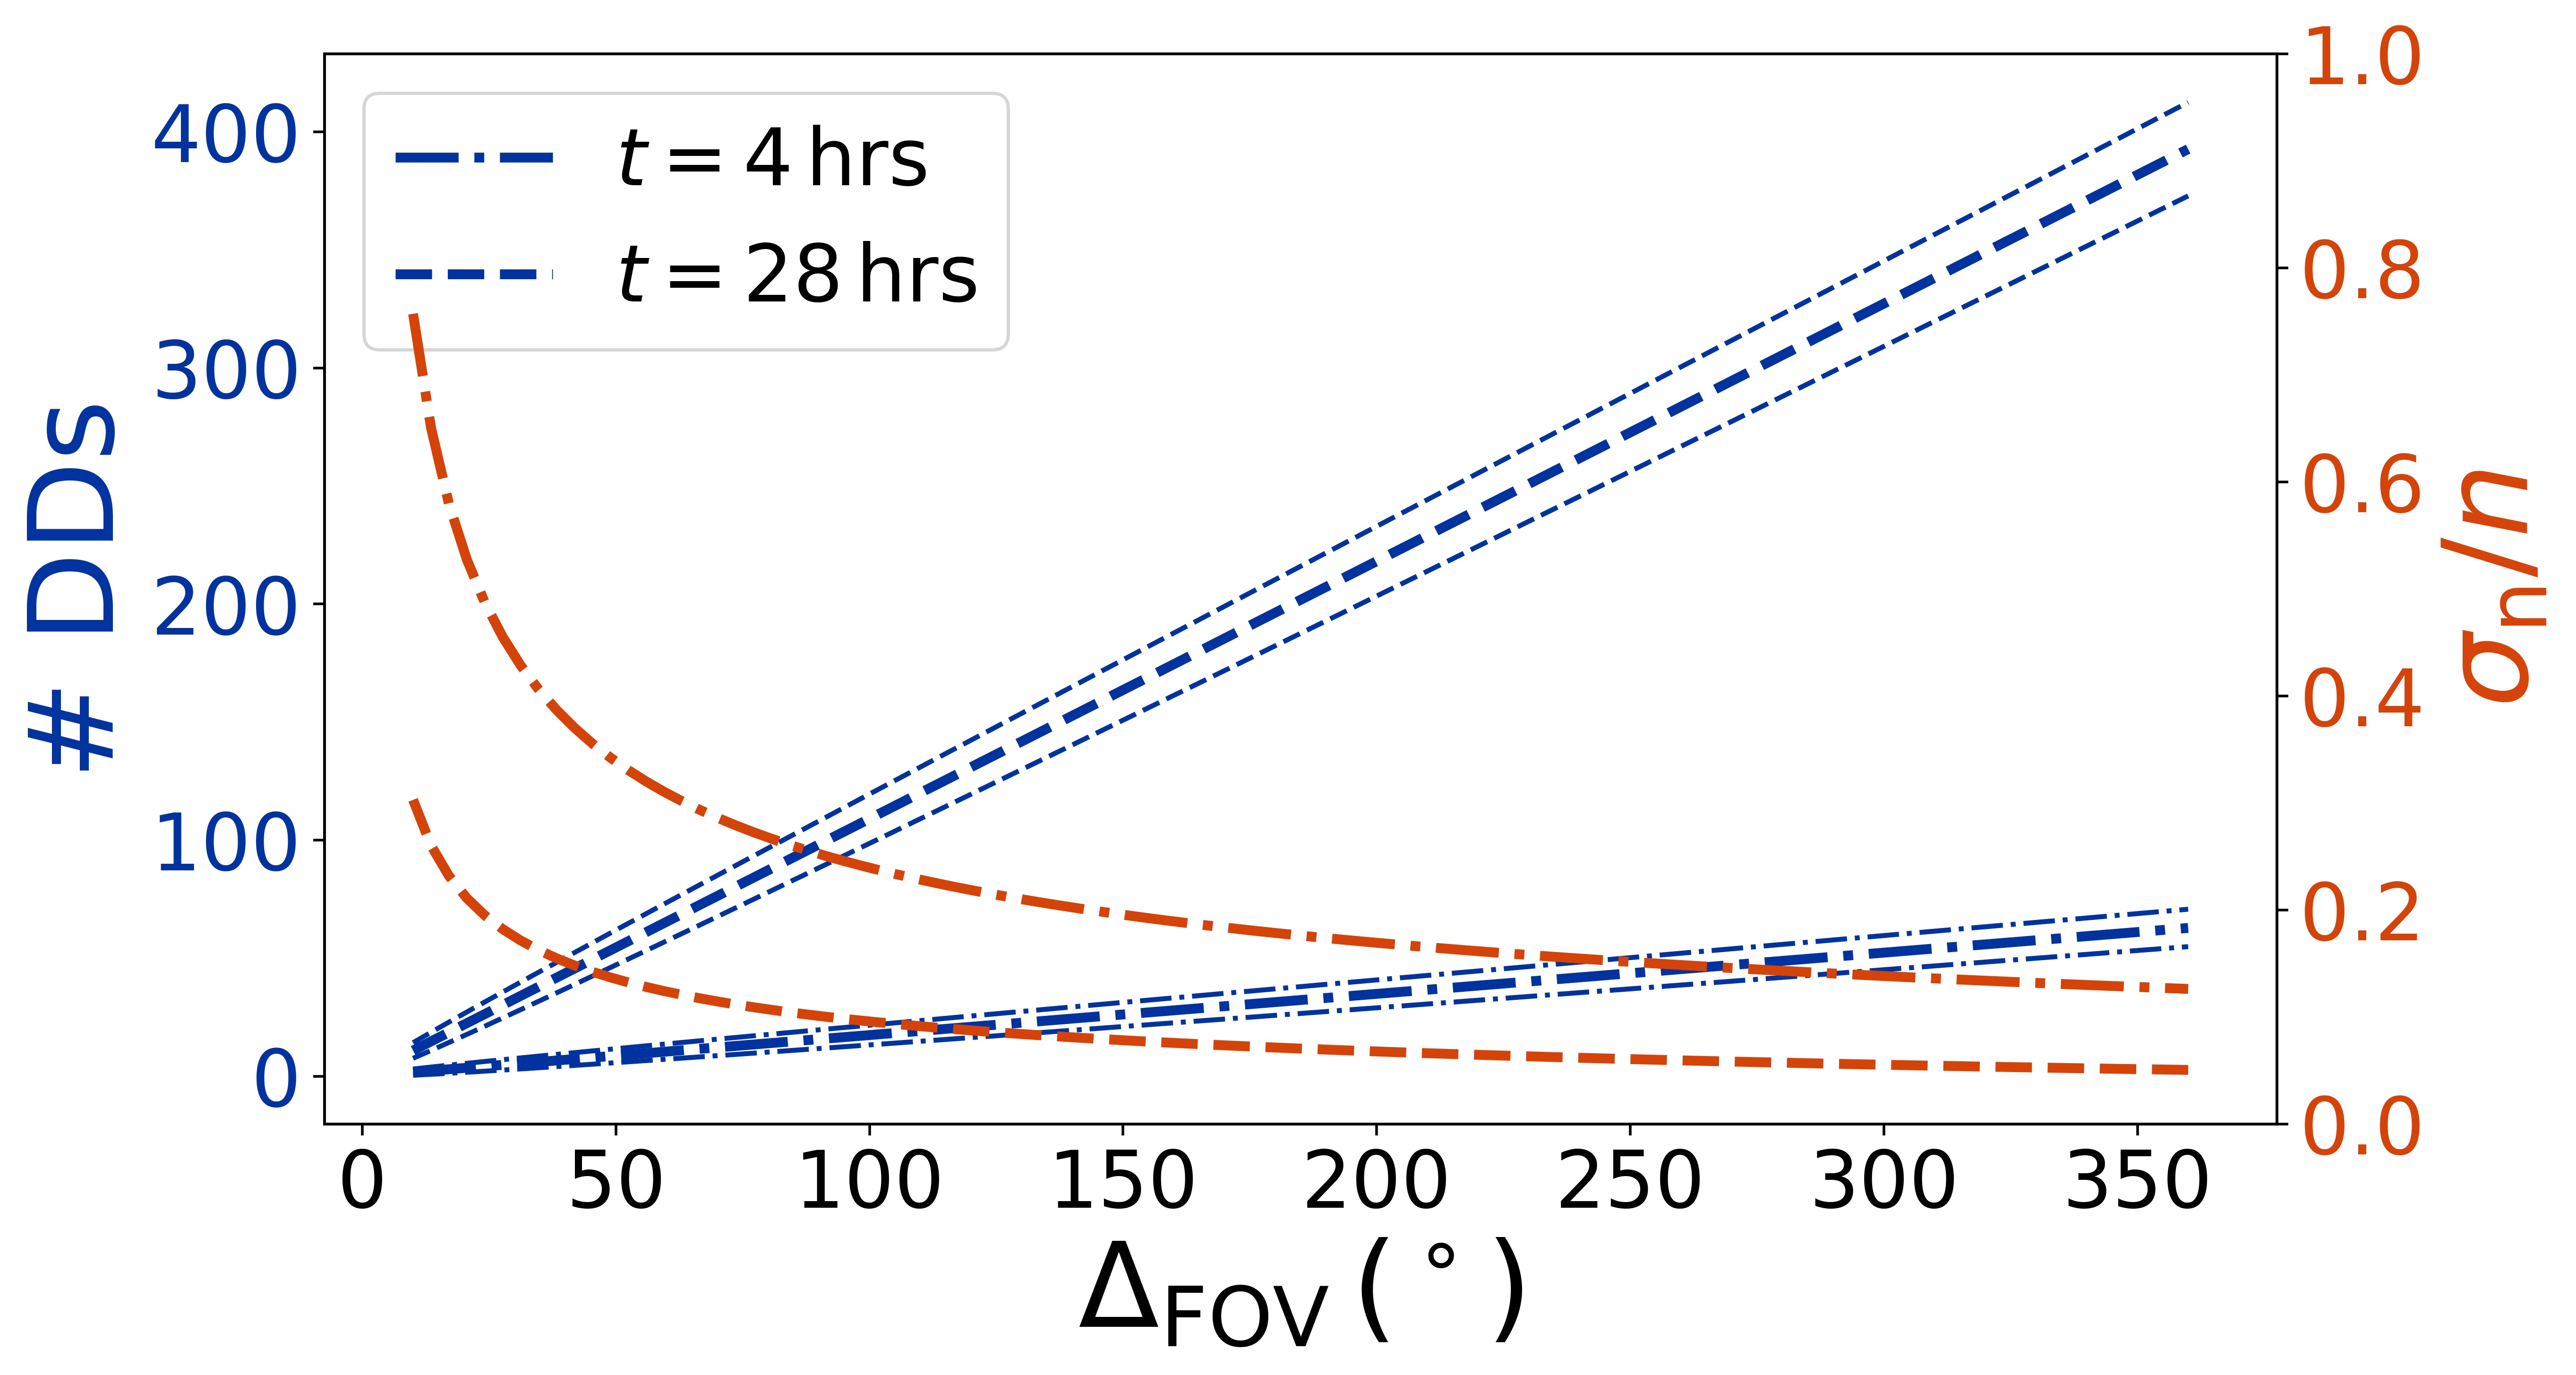
\includegraphics[width=\textwidth]{figures/DDs_vs_Delta.jpg}
    \caption{The expected range of dust devils recovered in an image as a function of field-of-view $\Delta_{\rm FOV}$ (filled blue region). The survey precision, $\sigma_N/N$ is shown as a dash-dot, orange line. The calculation here assumes $N = 0.03\,{\rm km^{-2}}$, $D = 10\,{\rm m}$, and $\alpha = 1\,{\rm mrad}$.}
    \label{fig:DDs_vs_Delta}
\end{figure}

% Usually, we would design our survey so that we achieve a sufficiently precise estimate for the quantity of physical significance $N$. In other words, we would require $\sigma_N/N < T$, some threshold. We can see that Equation \ref{eqn:sigma_N} provides the specific requirements to achieve the desired threshold. For instance, we can take some typical values from \citet{2006JGRE..11112S09G} and estimate what minimum angular resolution is required of our camera to achieve $T = 0.1$:
% \begin{equation}
%     \alpha < 2^{-1/2} T \left( n t \right)^{1/2} D\ \Delta_{\rm FOV}^{1/2} = 2^{-1/2} \left( 0.1 \right) \big[ \left( 0.05\,{\rm km^{-2}\ hr^{-1}} \right) \left( 1\,{\rm hr} \right) \big]^{1/2} \left( 10\,{\rm m} \right) \left( \pi/2\,{\rm rad} \right)^{1/2} \approx 0.2\,{\rm mrad}.
%     \label{eqn:alpha_example}
% \end{equation}
% Such an angular resolution is about ten times better than is usually achieved -- the MER Hazcams used for the survey in \citet{2006JGRE..11112S09G} had a resolution of $2\,{\rm mrad/pix}$ \citep{2003JGRE..108.8071M}.

Another application of Equation \ref{eqn:sigma_N} might instead involve assuming requiring a minimum survey accuracy $T = \sigma_N/N$ and asking, for a given camera field-of-view, what angular resolution is required. Figure \ref{fig:alpha_vs_Delta} shows the result: an accuracy of $T = 50\%$ can be achieved with $\Delta_{\rm FOV} = 150^\circ$ and a modest $\alpha = 1\,{\rm mrad}$ (i.e., resolving a dust devil with pixels across if the pixels each have a resolution of $0.3\,{\rm mrad\, pix^{-1}}$), again for $N = 0.03\,{\rm km^{-2}}$.

\begin{figure}
    \centering
    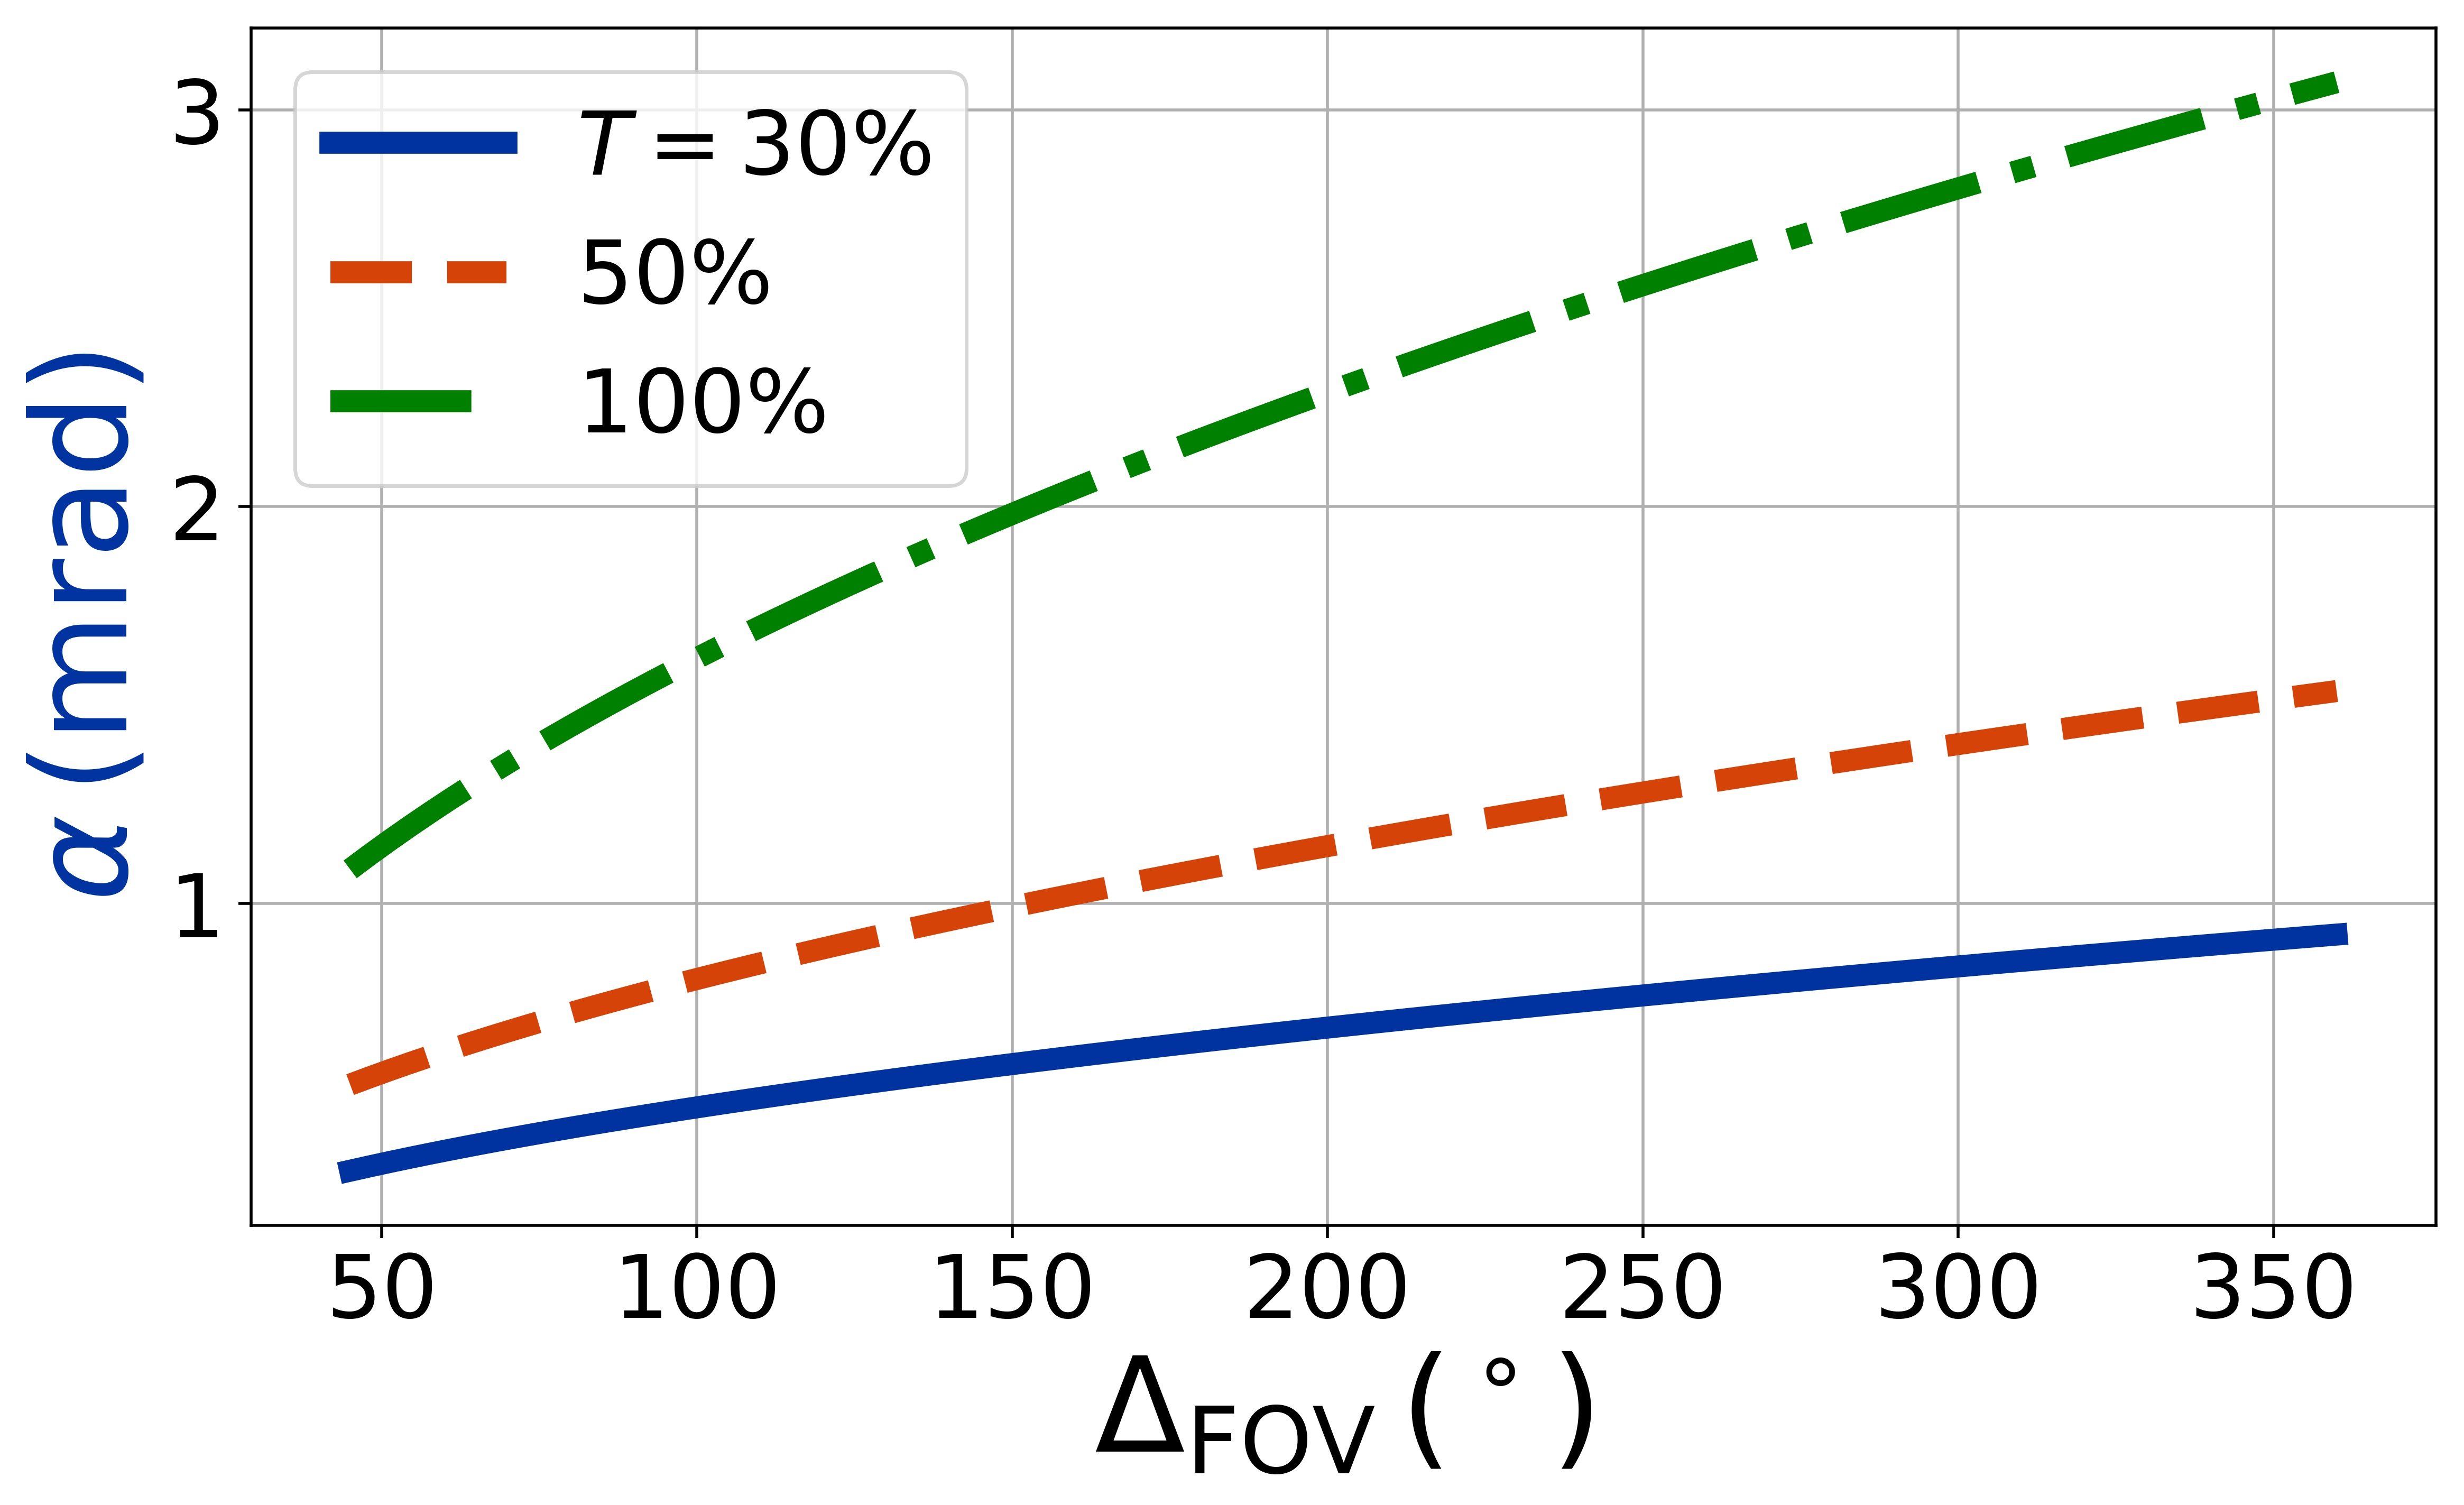
\includegraphics[width=\textwidth]{figures/alpha_vs_Delta.jpg}
    \caption{The $\Delta_{\rm FOV}$-$\alpha$ combinations required to achieve a desired survey accuracy $T = \sigma_N/N$. The calculation here assumes $N = 0.03\,{\rm km^{-2}}$ and $D = 10\,{\rm m}$.}
    \label{fig:alpha_vs_Delta}
\end{figure}

However, dust devils are usually active only for a few hours during each day (or sol on Mars) -- \citet{2006JGRE..11112S09G} found negligible activity before 9 a.m. LTST or after 5 p.m. LTST. Moreover, the occurrence rate itself seemed to evolve over the course of the active phase, increasing from $0.005\,{\rm km^{-2}\ hr^{-1}}$ early in the morning to  $0.05\,{\rm km^{-2}\ hr^{-1}}$ around noon. This mid-day peak agrees with meteorological predictions that dust devil activity should increase as the planetary boundary layer deepens with increasing surface heating \citep{doi:10.1029/2010RG000351}. Accurately estimating the occurrence rate requires a survey duration not longer than the timescale of variability, i.e., about an hour. Therefore, the 25-hours of survey required to recover $n = 0.05\,{\rm km^{-2}\ hr^{-1}}$ to 10\% accuracy would have to be spread into 1-hour surveys around noon spanning 25 sols. (And, of course, smaller occurrence rates would require additional time.) 

Similarly, \citet{2006JGRE..11112S09G} reported an occurrence rate that varied with season and $L_{\rm S}$. Assuming sufficient daily coverage to accurately capture the daily occurrence rate (i.e., a large enough value for $n t$), we can ask what $\Delta_{\rm FOV}$ might be required to recover the seasonal variability by looking at the expected variation in $n t$. From its peak in spring to the peak in summer, $n t$ dropped from $0.11\,{\rm km^{-2}}$ to $0.05\,{\rm km^{-2}}$, which would require a precision $\sigma_n/n \sim 0.5$. Solving Equation \ref{eqn:sigma_n} gives $\Delta_{\rm FOV} \approx 65^\circ$. Considering instead the maximum $\Delta_{\rm FOV} = 360^\circ$ and an areal occurrence $nt = 0.11\,{\rm km^{-2}}$ suggests we could recover dozens of 10-m wide dust devils. 

Importantly, all these calculations up till now have assumed a single dust devil diameter, $D$. In fact, dust devils span a range of diameters - \citet{2006JGRE..11112S09G} reported values between 2 and $276\,{\rm m}$, while orbital studies have reported devils hundreds of meters across \citep{2008Icar..197...39S}. However, the distribution of diameters appears to follow a steep power law, with an exponent between 1 and 2 \citep{2016SSRv..203..277L}. Consequently, the majority of devils reported in \citet{2006JGRE..11112S09G} lay between 10 and $20\,{\rm m}$, and so $n$ is dominated by devils in this range and the calculations presented so far may be considered reasonably representative. In addition, for a given angular resolution, larger dust devils can be recovered from farther away, an observational bias that has been previously pointed out \citep{2012Icar..219..556K, 2013Icar..226..964L}.

On the other hand, given that larger dust devils are less common, they may be intrinsically less likely to be recovered. Equation \ref{eqn:areal_occurrence_rate} may be adapted to allow for a distribution of dust devils by diameter by simply taking $n$ to represent the areal occurrence rate in a narrow range of diameters and $k$ to represent the number of devils observed within that same range of diameters. From Equation \ref{eqn:areal_occurrence_rate}, we can see that if $n$ were a steeply declining function of $D$ (e.g., $n \propto D^{-3}$), then the total number of devils recovered with smaller diameters would exceed the number with larger diameters in proportion to $D^{-1}$.

More than simply counting dust devils, a survey might consider also assessing dust devil dynamics. In their survey, \citet{2006JGRE..11112S09G} constructed 21-frame short movies of dust devils in order to estimate their advective motions. By tracking the motions of visually distinct eddies within dust devils, they also estimated vertical velocities, ranging from $0.2$ to $8.8\,{\rm m\ s^{-1}}$, and therefrom the atmospheric dust flux. 

In addition to sufficient time resolution (the movies analyzed in \citealt{2006JGRE..11112S09G} had a few seconds between frames), such an estimate requires sufficient angular resolution. Eddies within a dust devil span a range of sizes but all smaller than the host devil itself. In order for the motion of such an eddy to be resolvable, it must span a few pixels. At a minimum, the devil itself must be larger, occupying many times as pixels as the eddy, a minimum number of pixels $p_{\rm min}$.

In order for a dust devil with diameter $D$ to occupy $p_{\rm min}$ pixels, it must pass within a radial distance $r$ of the camera, given by 
\begin{equation}
    r \le \frac{D}{p_{\rm min} \alpha}.
    \label{eqn:encounter_distance}
\end{equation}
Passing within that radial distance requires the devil to pass through a pie-wedge area $A$ smaller than that corresponding to $r_{\rm max}$ but with the same opening angle $\Delta_{\rm FOV}$.

The time between encounters with such a dust devil $\tau_{\rm enc}$ can be estimated using $r$:
\begin{equation}
    \tau_{\rm enc} = \left( n A \right)^{-1} = \bigg[ \left( \frac{n \Delta_{\rm FOV}}{2} \right) \left( \frac{D}{p_{\rm min} \alpha } \right)^2 \bigg]^{-1}.
    \label{eqn:tau}
\end{equation}
For example, if we require a 10-m dust devil occupies 10 pixels (i.e., passes within $1\,{\rm km}$ of a camera with $\alpha = 1\,{\rm mrad}$ and $\Delta_{\rm FOV} = 65^\circ$), with $n = 0.05\,{\rm km^{-2}\ hr^{-1}}$, $\tau_{\rm enc} = 35\,{\rm hrs}$. In other words, a survey would require 35 hours of observation for such a small devil to pass so close to the camera. Assuming the same occurrence rate for 100-m devils, the same encounter distance would only require $\tau_{\rm enc} \approx 20\,{\rm min}$. However, the relative rarity of such large dust devils means encounters with such large devils would occur rarely. Figure \ref{fig:encounter_time} shows the encounter times for different diameters and various fields-of-view.

\begin{figure}
    \centering
    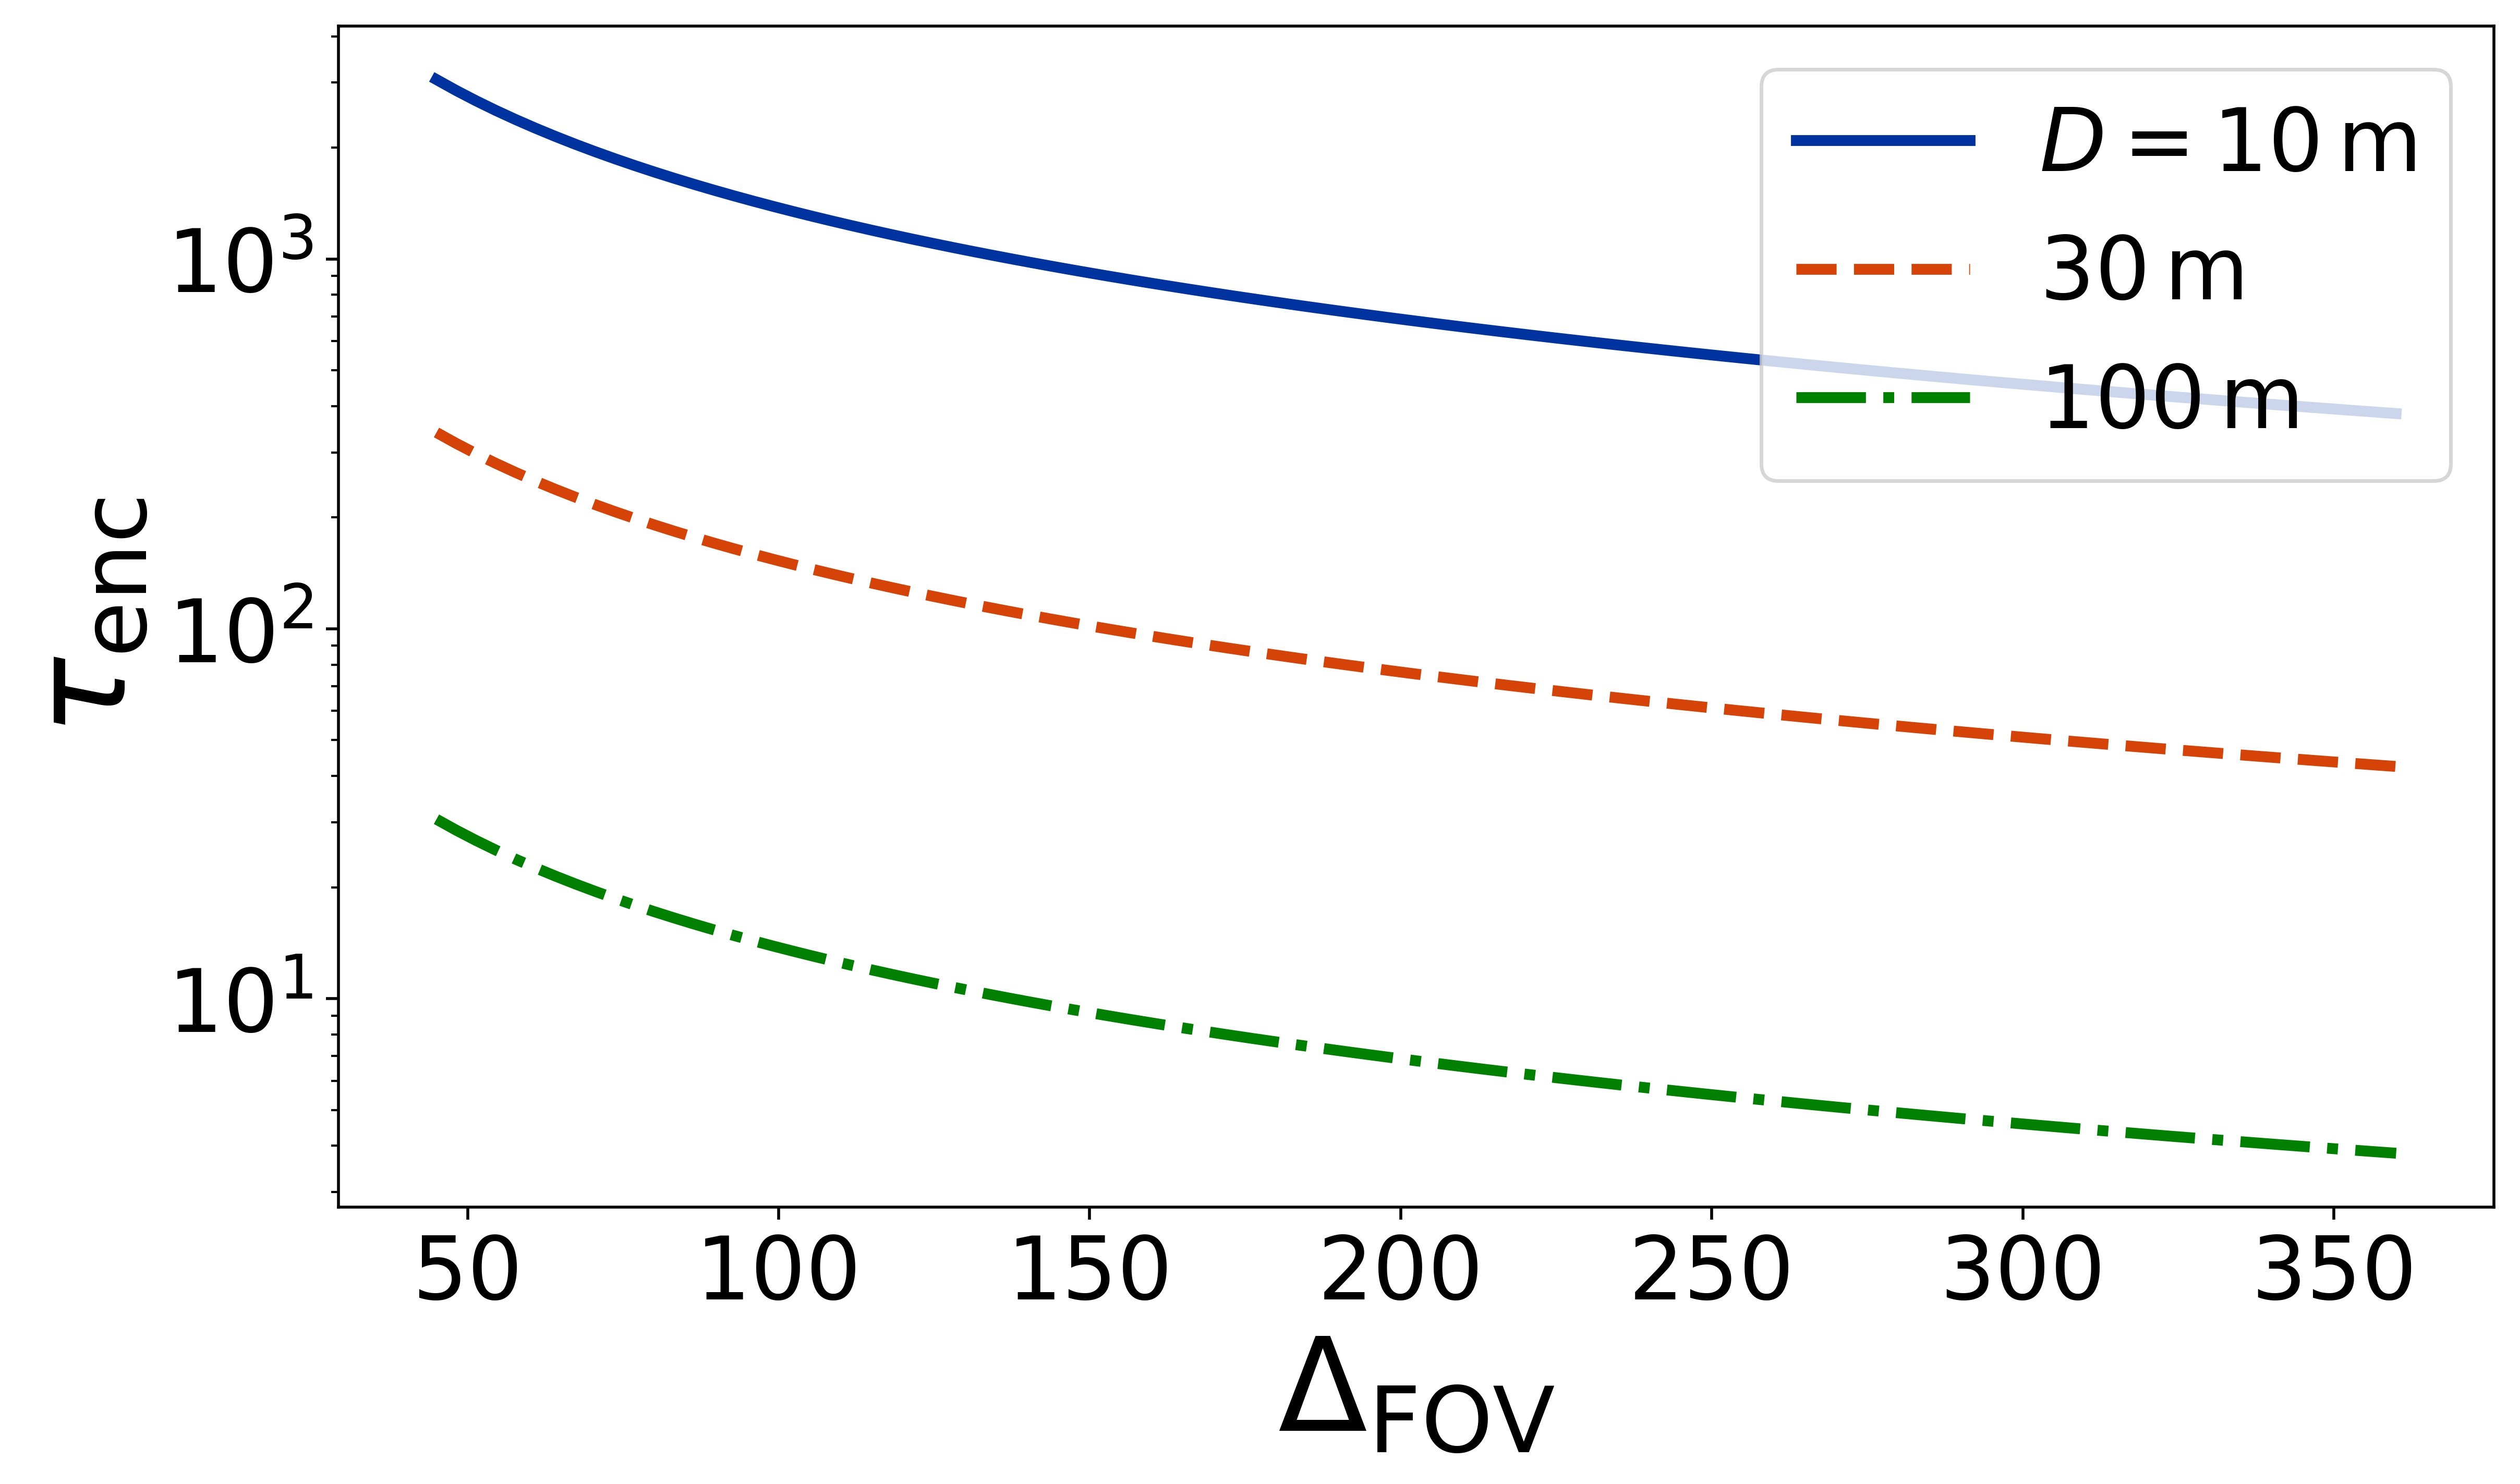
\includegraphics[width=\textwidth]{figures/encounter_time.jpg}
    \caption{The times between dust devil encounters close enough the devils can be clearly resolved for a range of diameters and fields-of-view $\Delta_{\rm FOV}$. All other parameters are the same as in previous figures.}
    \label{fig:encounter_time}
\end{figure}

\section{Assessing the Dust Flux}
Accurate recovery of the dust devil population, in particular the largest devils, may be critical to assess the contribution of dust devils to the martian dust budget. By tracking vertical velocities and optical depths within imaged dust devils, \citet{2006JGRE..11112S09G} estimated dust flux values $q$ for 300 devils, with values ranging between $3.95\times10^{−9}$ and $4.59\times10^{−4}\,{\rm kg\ m^{-2}\ s^{-1}}$ with an average $2.07\times10^{−5}\,{\rm kg\ m^{-2}\ s^{-1}}$, although no information is given regarding the dependence on diameter or any other parameter. Assuming this dust flux applies uniformly across diameter, it suggests the total dust contribution for a devil scales with that devil's areal footprint, i.e.~with $D^2$. We can use these values to explore how well we can estimate the dust flux for a given dust devil population.

Taking the areal occurrence rate of dust devils with a diameter within a small interval around $D$ as $dn/dD = n_0 D^{-\gamma}$ with $\gamma$ between 1 and 2 \citep{2016SSRv..203..277L}. (As before, the area of an individual dust devil does not factor into the areal occurrence rate.) This expression translates into a number of devils observed during a survey of duration $t$ and within a narrow range of diameters $dk/dD = \left( dn/dD \right) A_{\rm survey} t$. Taking the rate of dust mass lifting for a single devil as $Q = q\ \pi D^2$, we can estimate the population-weighted rate as 
\begin{equation}
    Q_{\rm tot} = \int_{D_{\rm min}}^{D_{\rm max}} \left( \frac{dk}{dD} \right) q\ \pi D^2 dD = \int_{D_{\rm min}}^{D_{\rm max}} n_0 D^{-\gamma} \left( \frac{t \Delta_{\rm FOV} D^2}{2 \alpha^2} \right) q \pi D^2\ dD.
    \label{eqn:dust_lifted}
\end{equation}
Although the dust flux $q$ likely depends on $D$ itself, the dependence is unknown, and so for simplicity, we will assume $q = {\rm const.}$, yielding 
\begin{equation}
    \langle Q \rangle = \pi q n_0 \left( \frac{t \Delta_{\rm FOV}}{2 \alpha^2} \right) \left( \frac{D_{\rm max}^{5 - \gamma} - D_{\rm min}^{5 - \gamma}}{5 - \gamma} \right) \approx \left( \frac{ \pi q n_0 }{2 \left( 5 - \gamma \right)} \right) \left( \frac{t \Delta_{\rm FOV}}{\alpha^2} \right) D_{\rm max}^{5 - \gamma},
    \label{eqn:solved_dust_lifted}
\end{equation}
with $\gamma < 5$ and $D_{\rm min} \ll D_{\rm max}$. For a representative estimate, we can take $q = 2.07\times10^{−5}\,{\rm kg\ m^{-2}\ s^{-1}}$, $n_0 = 0.05\,{\rm km^{-2}\ hr^{-1}}$, $\gamma = 1$, $t = 25\,{\rm hrs}$, $\Delta_{\rm FOV} = 65^\circ$, $\alpha = 1\,{\rm mrad}$, and $D_{\rm max} = 100\,{\rm m}$, giving an estimate $\langle Q \rangle \approx 4 {\rm g\ hr^{-1}}$.

\section{Meteorological Time-Series}
Analyzing the pressure time-series from the Insight lander, \citet{2020arXiv200501134S} reported an unprecedented number of vortex detections, 9,019 in all. Their detection scheme was simple: they sought dips in the pressure time-series $\Delta P$ with a magnitude greater than $0.3\,{\rm Pa}$ of a rolling average within a window 1000-seconds wide. Figure \ref{fig:vortex_illustration} illustrates the $\Delta P$-values and sol of all the vortices reported, along with the profiles of some examples.

The earlier and more accurately a lander could register an encounter with such a vortex, the better the vortex could be probed by other instruments on the lander. To this end, we analyzed the Insight pressure time-series to explore a variety of strategies to detect the vortices in the incipient stages of the encounter. 

\begin{figure}
    \centering
    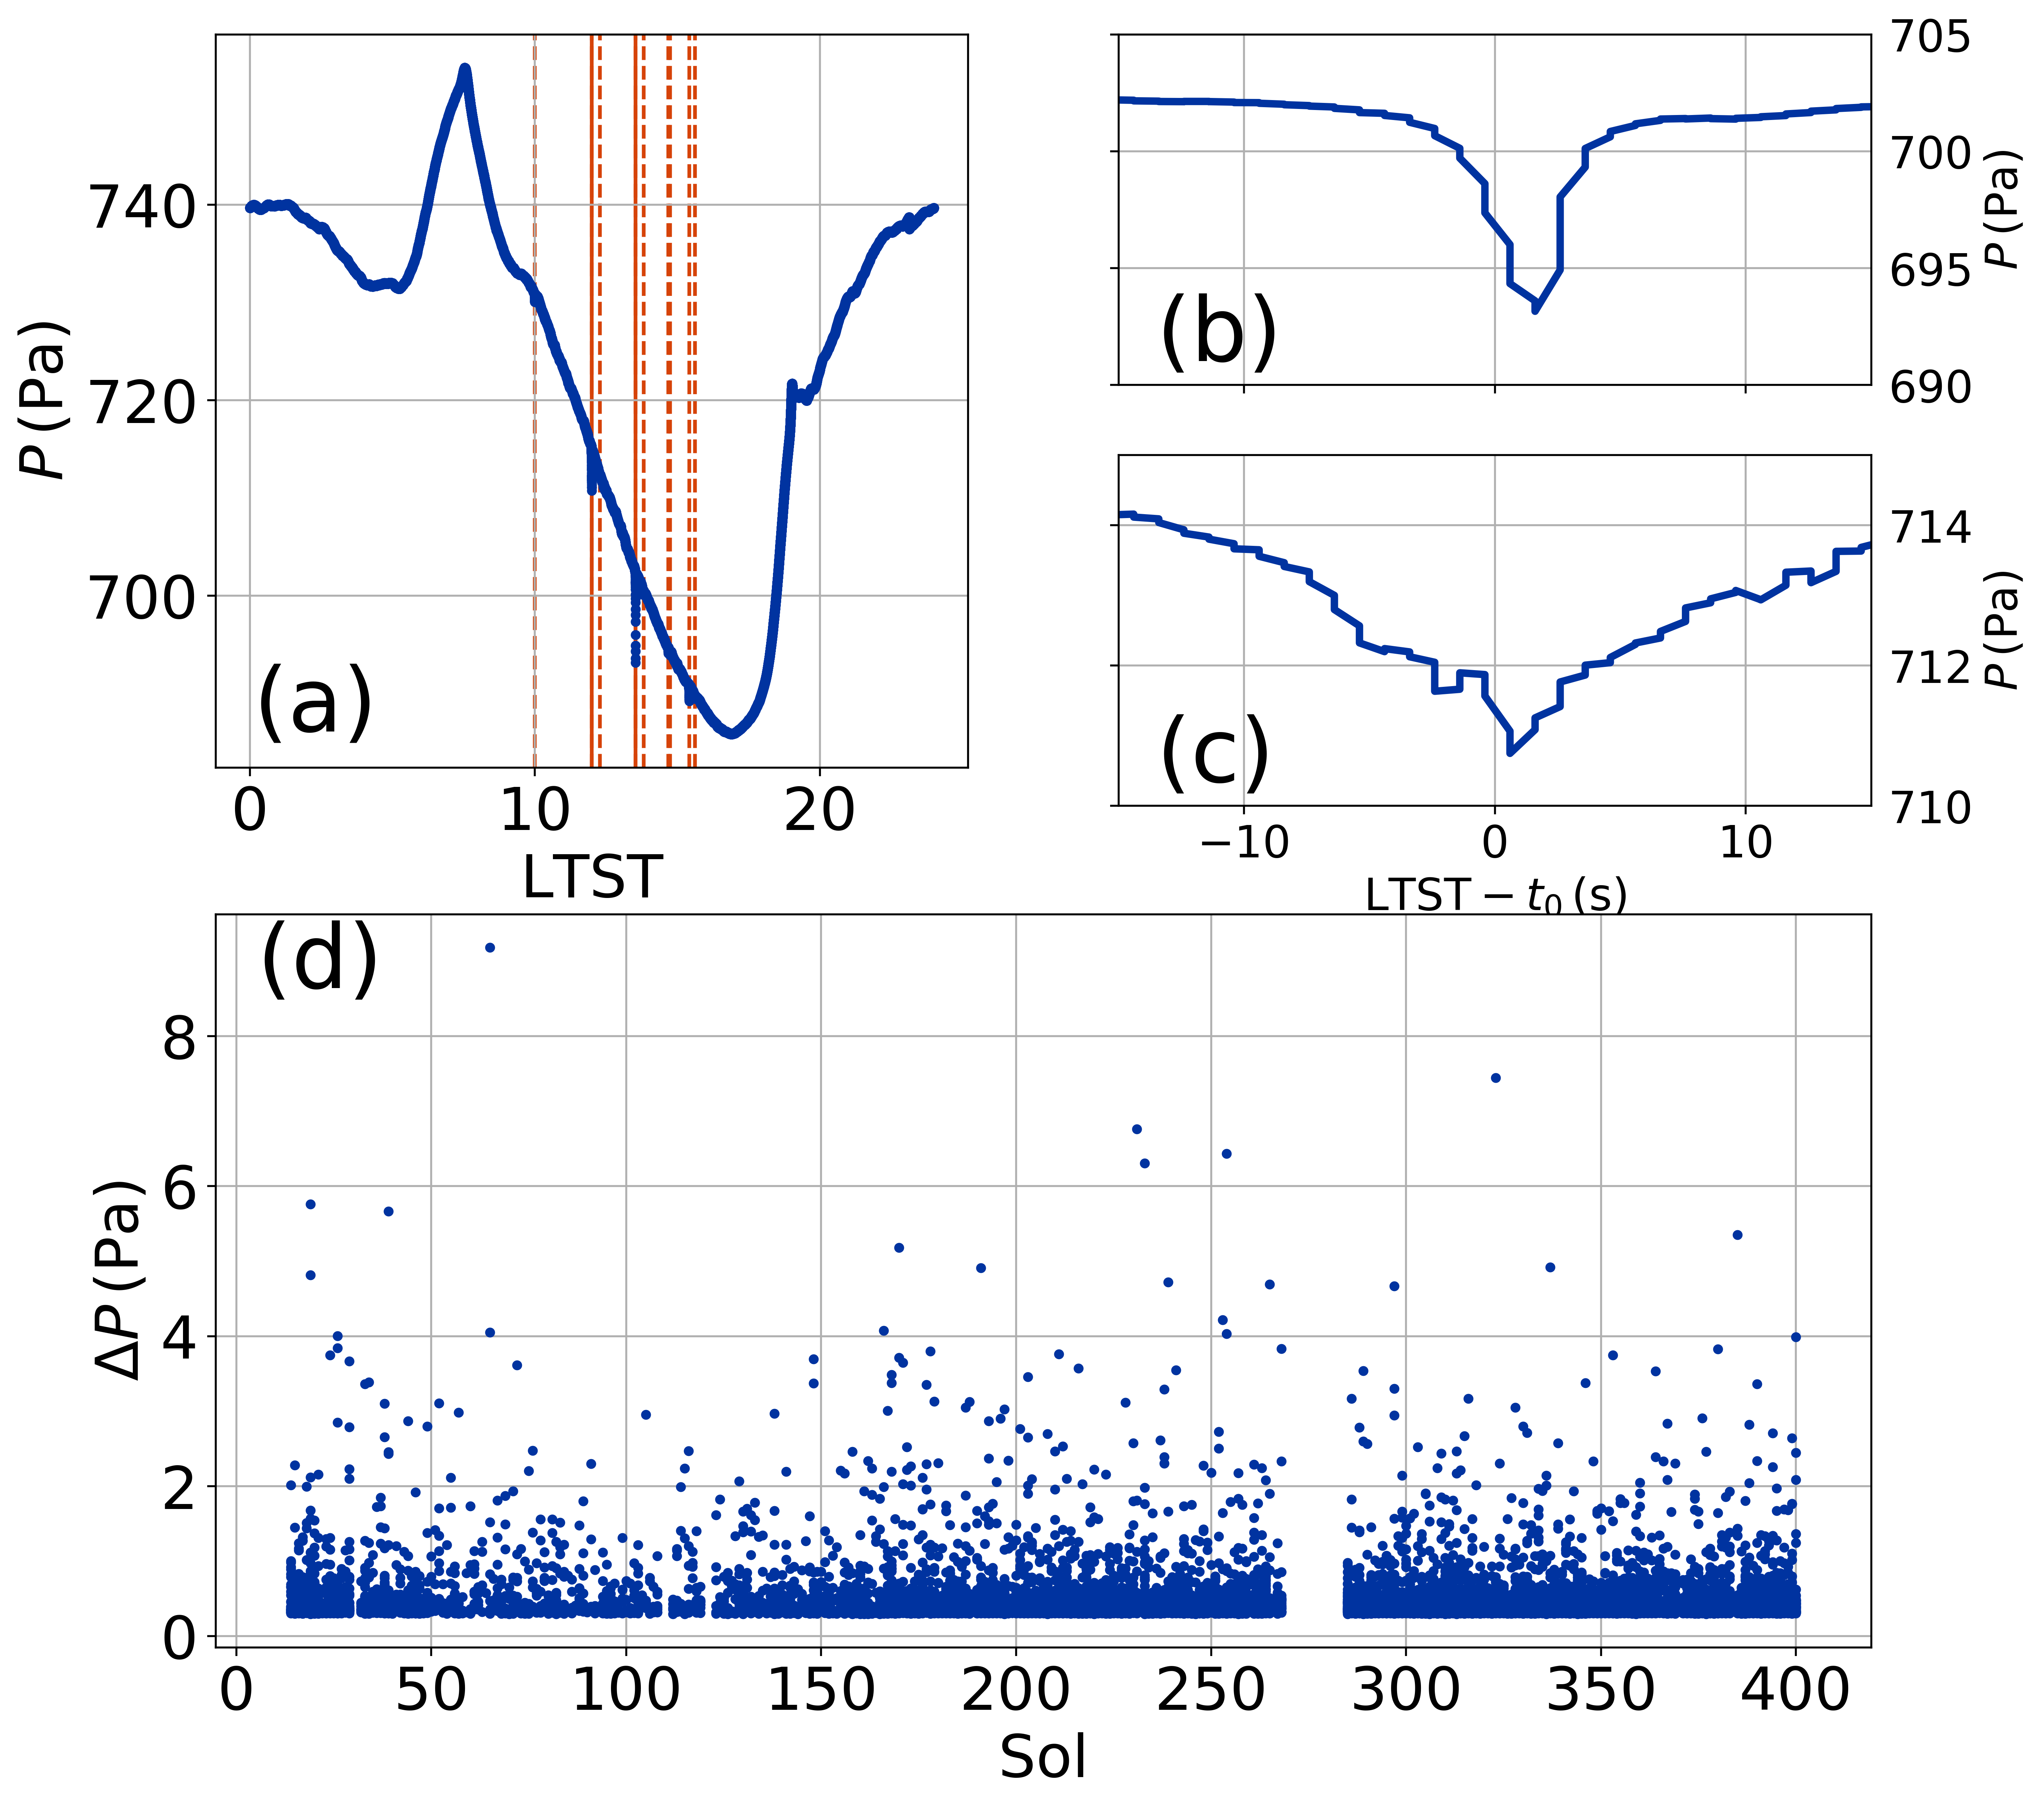
\includegraphics[width=\textwidth]{figures/vortex_illustration.png}
    \caption{(a) Insight pressure time-series from sol 65 shown as blue dots. The solid and dashed orange vertical lines show the positions of vortices reported in \citet{2020arXiv200501134S}. (b) The deepest ($\Delta P = 9\,{\rm Pa}$) vortex with time centered on the central time ($t_0$) reported in \citet{2020arXiv200501134S} and highlighted in (a) as the rightmost solid orange line. (c) A more typical vortex ($\Delta P = 4\,{\rm Pa}$) (leftmost solid orange line in (a)). (d) All vortex detections from \citet{2020arXiv200501134S}.}
    \label{fig:vortex_illustration}
\end{figure}

\acknowledgments

%% To help institutions obtain information on the effectiveness of their 
%% telescopes the AAS Journals has created a group of keywords for telescope 
%% facilities.
%
%% Following the acknowledgments section, use the following syntax and the
%% \facility{} or \facilities{} macros to list the keywords of facilities used 
%% in the research for the paper.  Each keyword is check against the master 
%% list during copy editing.  Individual instruments can be provided in 
%% parentheses, after the keyword, but they are not verified.

\vspace{5mm}
\facilities{}

%% Similar to \facility{}, there is the optional \software command to allow 
%% authors a place to specify which programs were used during the creation of 
%% the manuscript. Authors should list each code and include either a
%% citation or url to the code inside ()s when available.

\software{}

%% Appendix material should be preceded with a single \appendix command.
%% There should be a \section command for each appendix. Mark appendix
%% subsections with the same markup you use in the main body of the paper.

%% Each Appendix (indicated with \section) will be lettered A, B, C, etc.
%% The equation counter will reset when it encounters the \appendix
%% command and will number appendix equations (A1), (A2), etc. The
%% Figure and Table counter will not reset.

\appendix

\section{Vortex Recovery Statistics}
In this section, we describe our analysis of our vortex recovery statistics. We explored the effects of the mean boxcar filter on both the time-series scatter but also on the detected vortices, as well as the effectivenesss of our matched filter approach.

For our study here, the mean boxcar filter  acts as high-pass filter on the APSS pressure time-series and, in principle, should induce little distortion on signals much narrower than the filter window size $W$. However, some vortices have quite long durations (many tens of seconds), and so they may be prone to distortion if we used a small enough window. As a measure of this distortion, we can calculate how much less deep a vortex profile would appear after applying the filter by calculating the convolution of a boxcar function $B(t)$ against a Lorentzian profile, where $B(t)$ is $1/W$ within the window ($-W/2 < t < +W/2$):
\begin{equation}
    \Delta P_{\rm obs}^\prime = \int_{t = -W/2}^{+W/2} \left( \frac{1}{W} \right) \left( \frac{-\Delta P_{\rm obs}}{1 + \left( \frac{t}{\Gamma_{\rm obs}/2} \right)^2} \right) = -\left( \frac{\Delta P_{\rm obs} \Gamma_{\rm obs}}{W}\right) \tan^{-1} \left( \frac{W}{\Gamma_{\rm obs}} \right), \label{eqn:tophat_convolution}
\end{equation}
where we have taken the Lorenztian to be center at $t_0 = 0$ and $\Delta P_{\rm obs}^\prime$ represents the distorted profile depth. Figure \ref{fig:Pobsprime-sigmaP_vs_W}(a) shows the result: for windows more than 100 times the profile's original width (i.e., $W/\Gamma_{\rm obs} > 10^2$), the profile width is more than 98\% of its original value, indicating minimal distortion. 

Of course, the narrower the window, the more effectively we can reduce the long-term variations in the time-series that may otherwise obscure the vortices. To explore that effect, we applied mean boxcar filters of various widths $W$ to each sol's pressure time-series and then estimated the resulting scatter via $1.4826\ \times$ the median absolute deviation \citep{doi:10.1080/01621459.1993.10476408}. Figure \ref{fig:Pobsprime-sigmaP_vs_W}(b) shows the resulting range of values: the time-series for sol 435 showed the largest scatter for any value of $W$, while that for sol 269 showed the smallest. The time-series for sol 392 exhibited values near the median for each given $W$. 

\begin{figure}
    \centering
    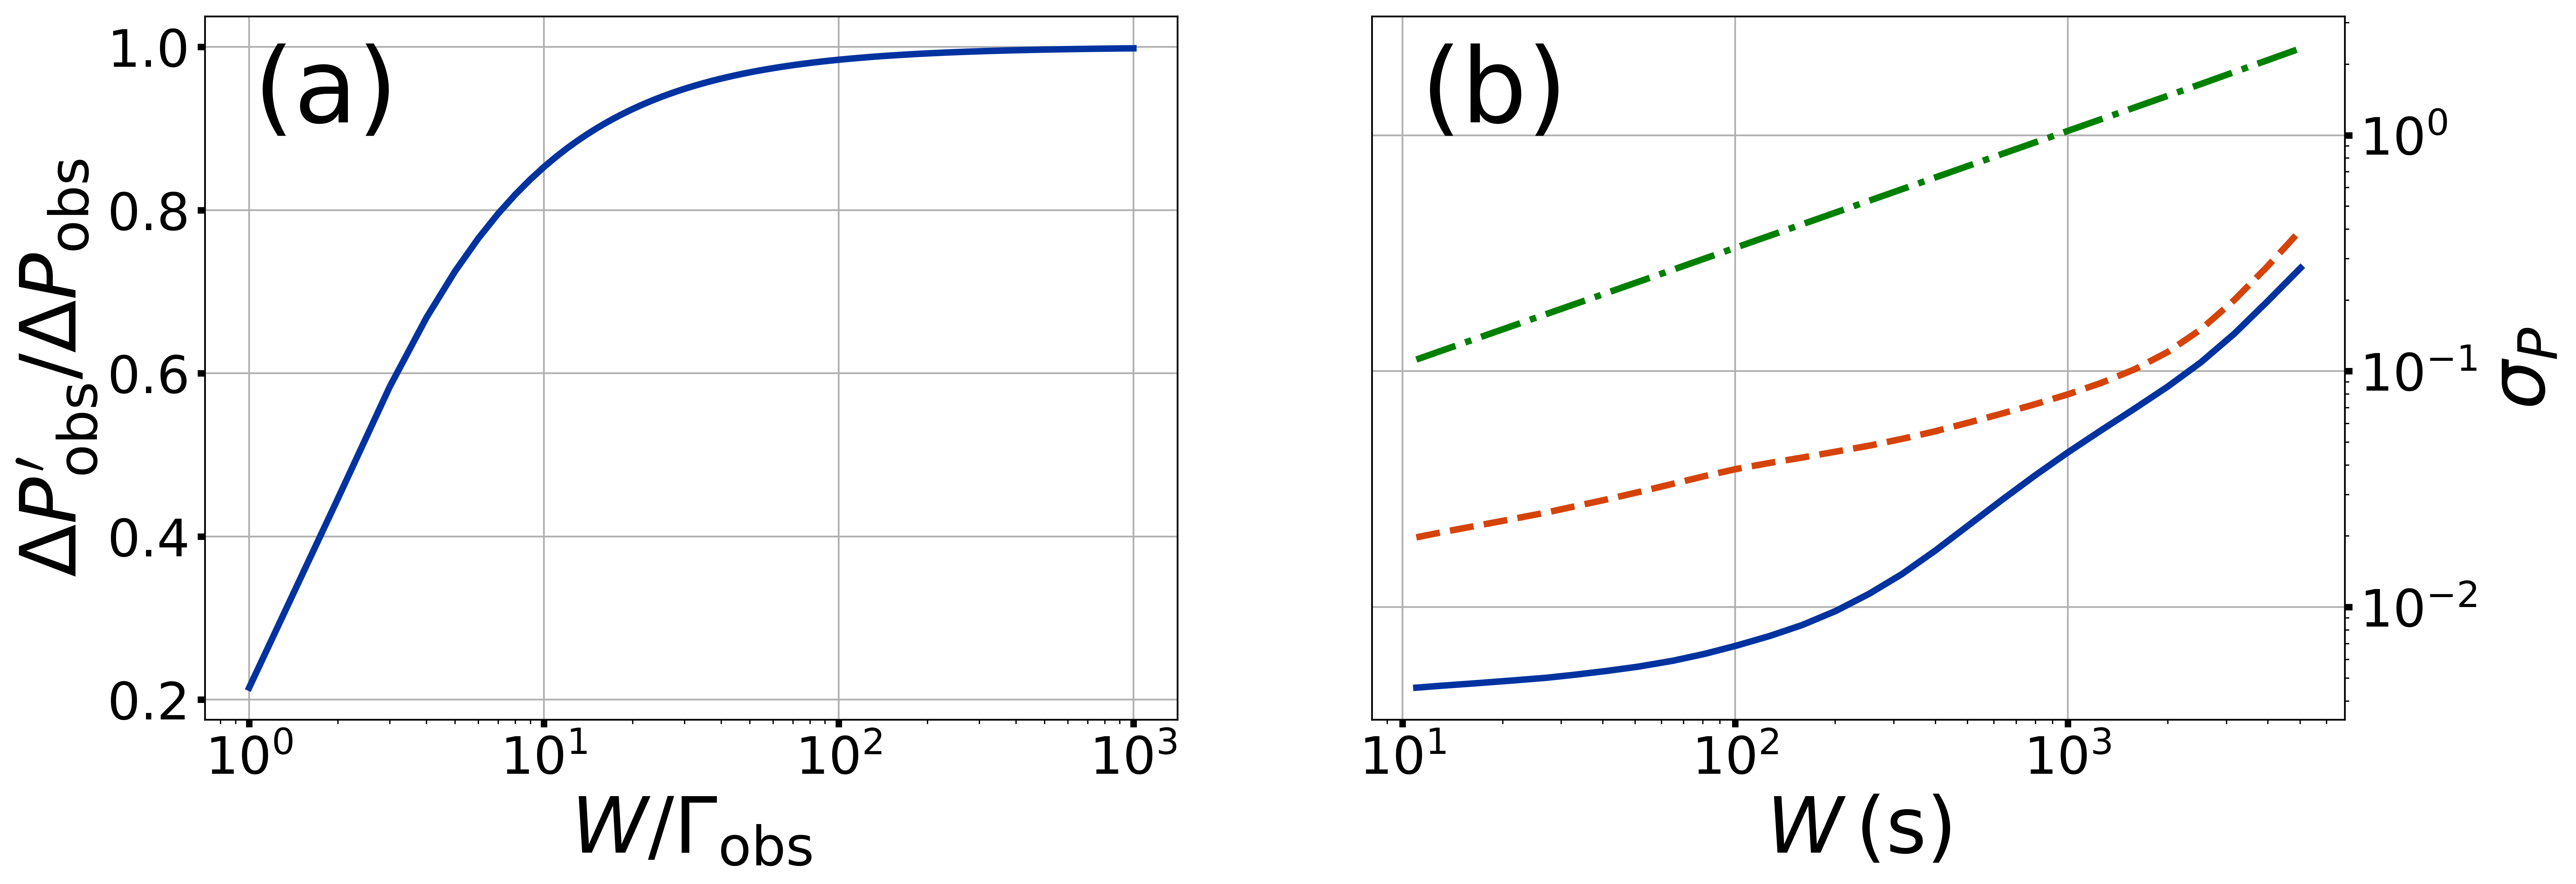
\includegraphics[width=\textwidth]{figures/Pobsprime-sigmaP_vs_W.png}
    \caption{(a) Comparing the pressure excursion observed before $\Delta P_{\rm obs}$ application of the mean boxcar filter and after $\Delta P_{\rm obs}^\prime$ as a function of the width of the filter $W$ and of the vortex signal $\Gamma_{\rm obs}$. (b) Scatter in the pressure time-series $\sigma_P$ for the sol with the largest (sol 435) and least (sol 269) values as a function of the window size $W$ for the mean boxcar filter. Sol 392 has scatter close the median value for all sols. }
    \label{fig:Pobsprime-sigmaP_vs_W}
\end{figure}

Finally, we must interpret these results in terms of our ability to recover vortices using our matched filter approach. In particular, we need to know the best shape for the matched filter: too narrow a filter might miss wider vortex profiles, while a wide filter could average out narrow profiles. To that end, we generated many synthetic time-series with the same sampling as the APSS time-series and with white noise with a wide range of variances $\sigma_\text{P}^2$. Into these time-series, we injected a vortex signal with a known depth and width. Then, we applied our matched filter to see the range of values we retrieved for the convolution of the filter against the synthetic time-series (which we also normalized to its 

\begin{figure}
    \centering
    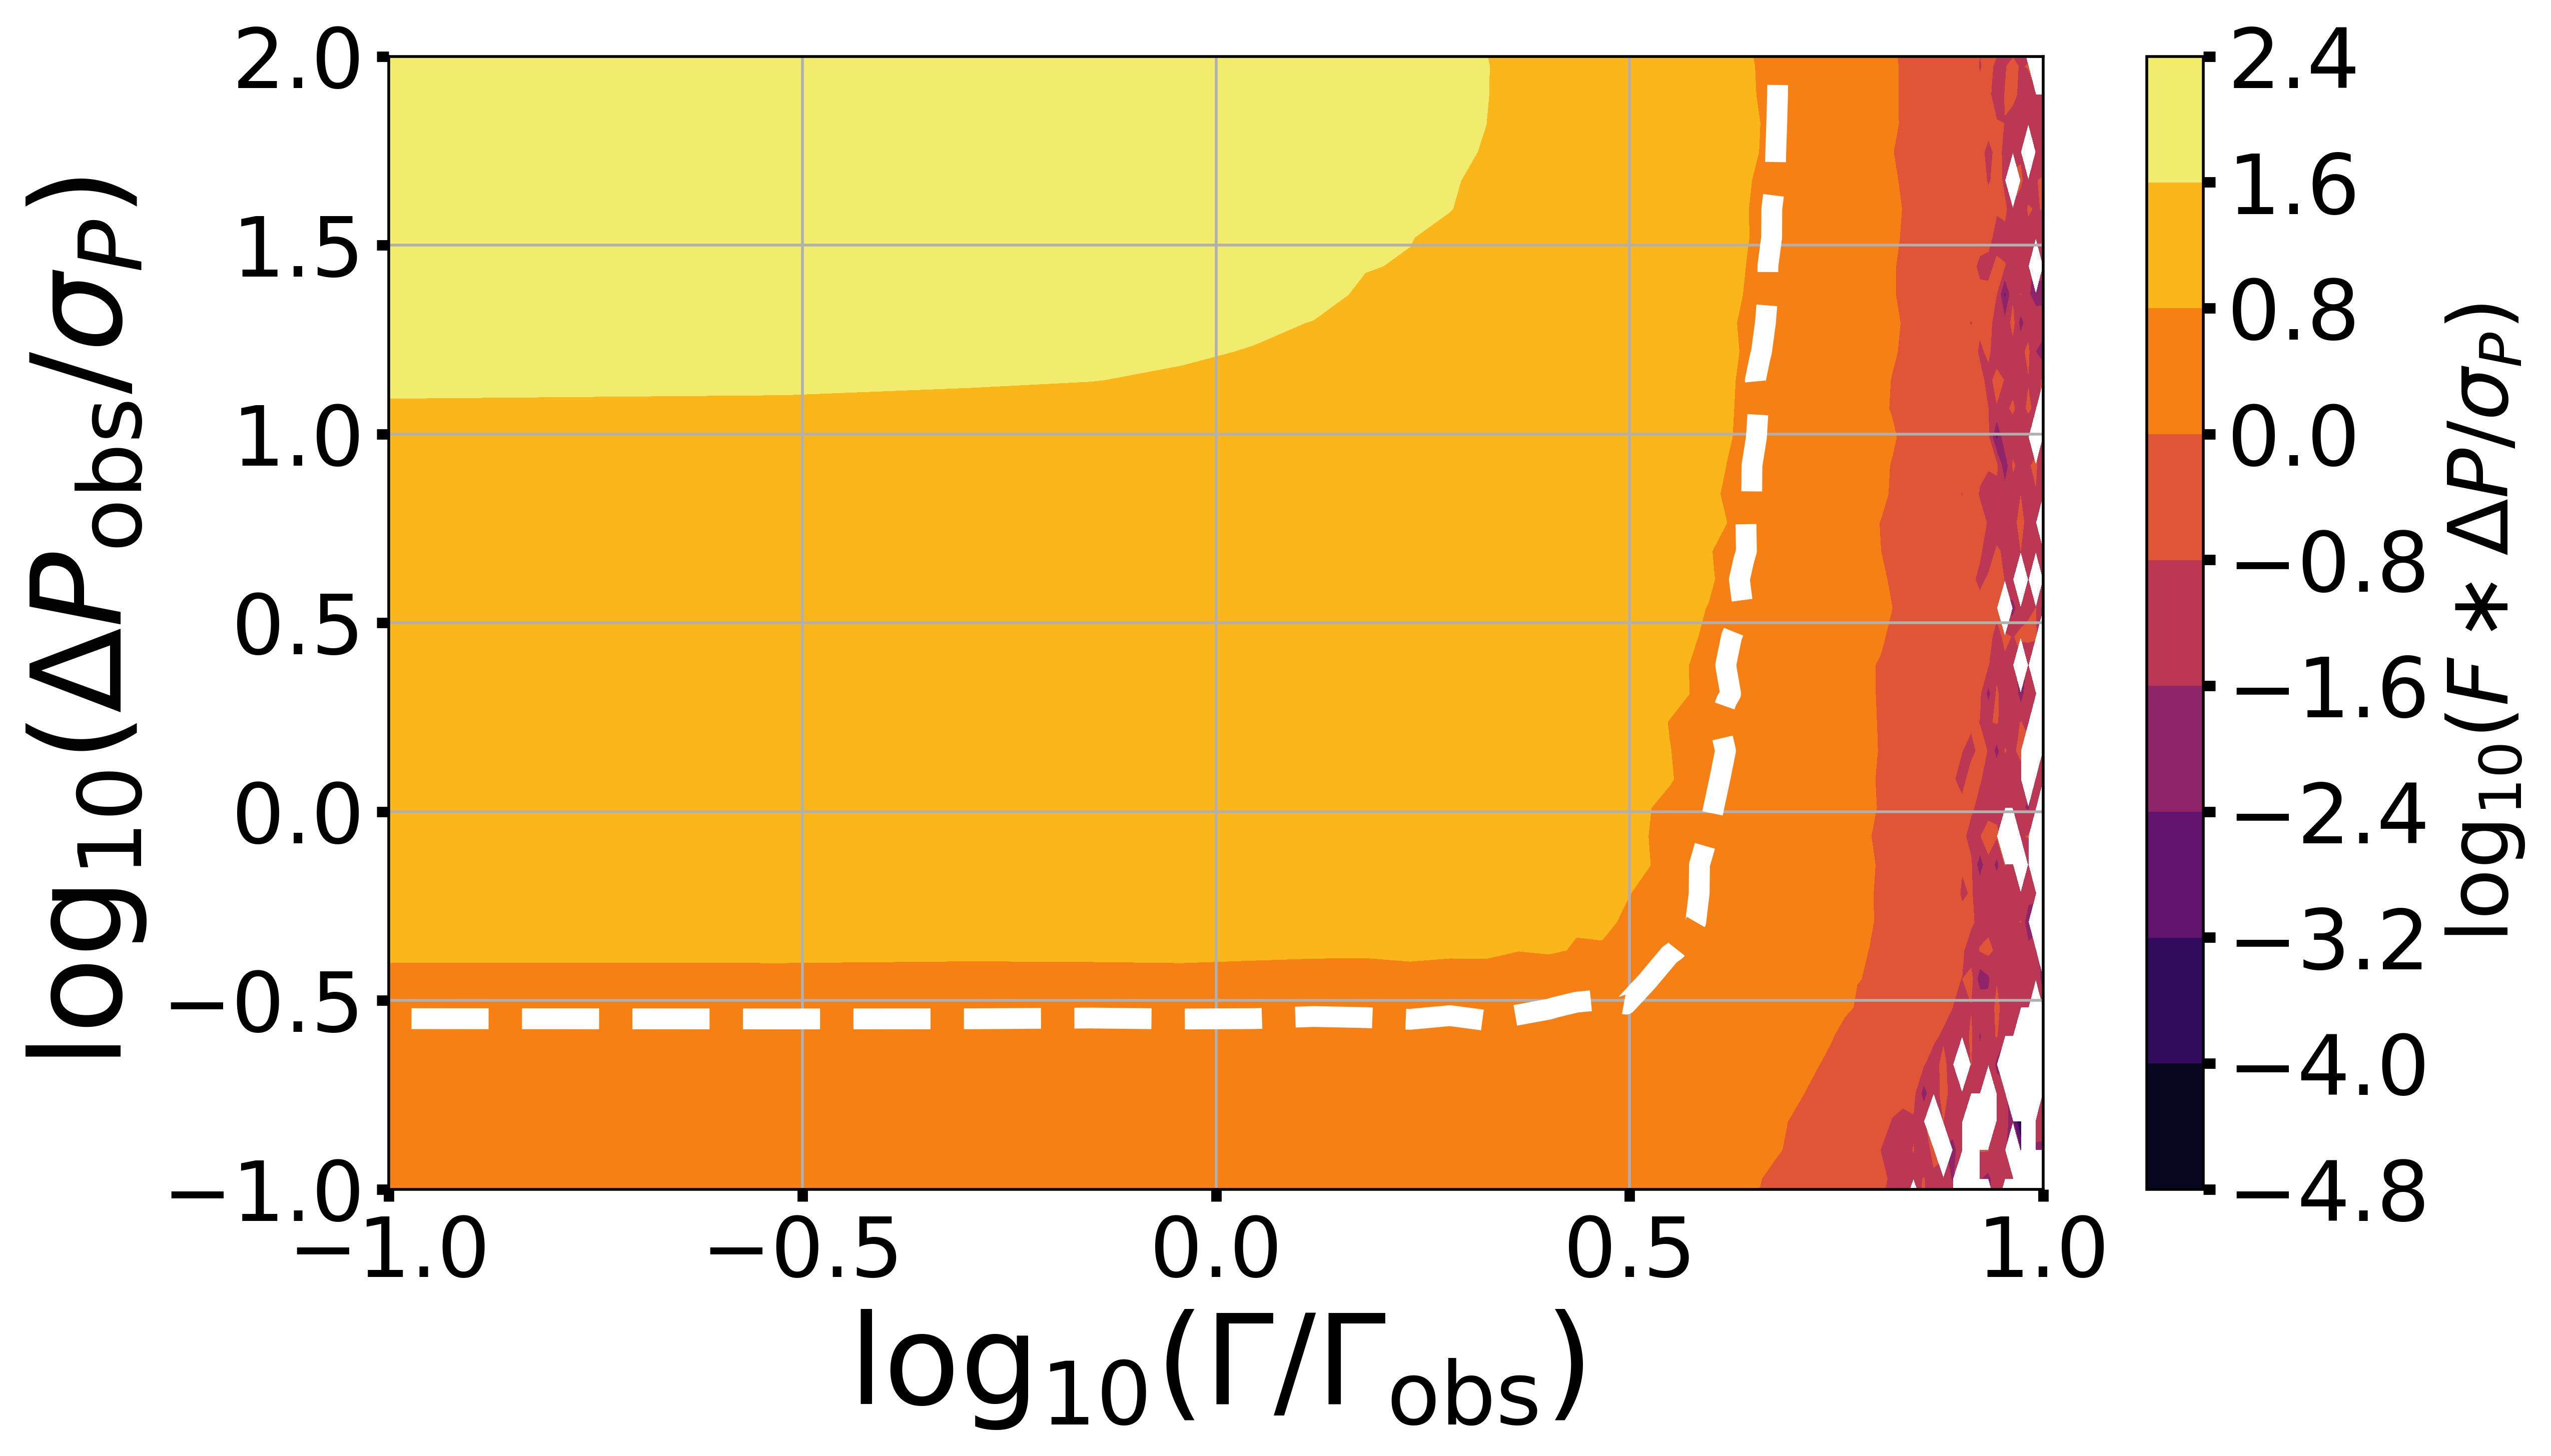
\includegraphics[width=\textwidth]{figures/vortex_recovery.png}
    \caption{How effectively a convolution of the filtered/normalized pressure time-series with the matched filter ($F\ast \Delta P\sigma_P$) recovers a vortex. The vortex has a known depth $\Delta P_\text{obs}$ and width $\Gamma_\text{obs}$ and is embedded in a synthetic time-series with white noise of variance $\sigma_\text{P}^2$. The matched filtered has a width $\Gamma$. The dashed, white line shows the threshold for detection used in this study ($F\ast \Delta P\sigma_P \geq 5$). In principle, vortices with values of $\Delta P_\text{obs}\sigma_P$ and $\Gamma/\Gamma_\text{obs}$ above and to the left of that line could be recovered.}
    \label{fig:vortex_recovery}
\end{figure}

% 2020 May 9 - Check notes in notepad from today's date
% \section{Effects of Undersampling the Dust Devil Profile}
% With too low a sampling frequency, the pressure profile for a dust devil will be undersampled, potentially distorting the inferred profile shape and depth. Fourier analysis of the pressure profile can show the dependence of the distortion on the angular sampling frequency $\omega$.

% We start by assuming a Lorentzian profile $L(t)$ in time $t$ for the dust devil:
% \begin{equation}
%     L(t) = -\frac{\Delta P}{1 + \left( t/\Gamma \right)^2},
%     \label{eqn:appendix_lorentzian}
% \end{equation}{}
% where $\Delta P$ is the profile depth and $\Gamma$ its duration. The Fourier transform of this profile $F(\omega)$ is 
% \begin{equation}
%     F(\omega) = -\pi \Delta P\ \Gamma e^{-|\omega| \Gamma}.
%     \label{eqn:appendix_lorentzian_fourier}
% \end{equation}{}

% If we now imagine that we undersampled the profile using frequencies below some maximum, $\omega \le \omega_{\rm max}$, then we can estimate the resulting distorted profile $L^\prime(t)$ by taking the inverse, partial Fourier transform of $F(t)$, i.e.
% \begin{equation}
%     L^\prime(t) \equiv \int_{\omega = -\omega_{\rm max}}^{\omega_{\rm max}}\ \left( -\pi \Delta P \Gamma e^{-|\omega| \Gamma}\right) \ \left( \frac{e^{+i\omega t}\ d\omega}{2 \pi} \right)
%     = L(t) \bigg[ 1 - \left( \cos \left( \omega_{\rm max} t \right) - \left( \frac{t}{\Gamma} \right) \sin \left( \omega_{\rm max} t \right) \right) e^{-\omega_{\rm max} \Gamma} \bigg].
%     \label{eqn:appendix_inverse_fourier}
% \end{equation}{}

% We expect the register the maximum (in magnitude) pressure excursion at the center of the profile, i.e. $L(t = 0) = \Delta P$, and so to estimate the incorrect profile depth $\Delta P^\prime$ arising from this distorted profile, we can evaluate $L^\prime(t)$ at the same time, giving:
% \begin{equation}
%     \Delta P^\prime = \Delta P \left( 1 - e^{-\omega_{\rm max}\Gamma} \right).
% \end{equation}{}
% The distortion decreases rapidly with $\omega_{\rm max}$, and for a sampling frequency of, for example, $2\,{\rm Hz}$ ($\omega_{\rm max} = 2\pi \times (2\,{\rm Hz})$) and a very narrow profile $\Gamma = 0.5\,{\rm s}$, $\Delta P^\prime$ is only 0.2\% different from $\Delta P$.

\bibliography{sample63}{}
\bibliographystyle{aasjournal}

%% This command is needed to show the entire author+affiliation list when
%% the collaboration and author truncation commands are used.  It has to
%% go at the end of the manuscript.
%\allauthors

%% Include this line if you are using the \added, \replaced, \deleted
%% commands to see a summary list of all changes at the end of the article.
%\listofchanges

\end{document}

% End of file `sample63.tex'.